\subsection{Movement and Diffusion}

\begin{figure}[h]
  \centering
  \begin{minipage}[t]{0.3\textwidth}
    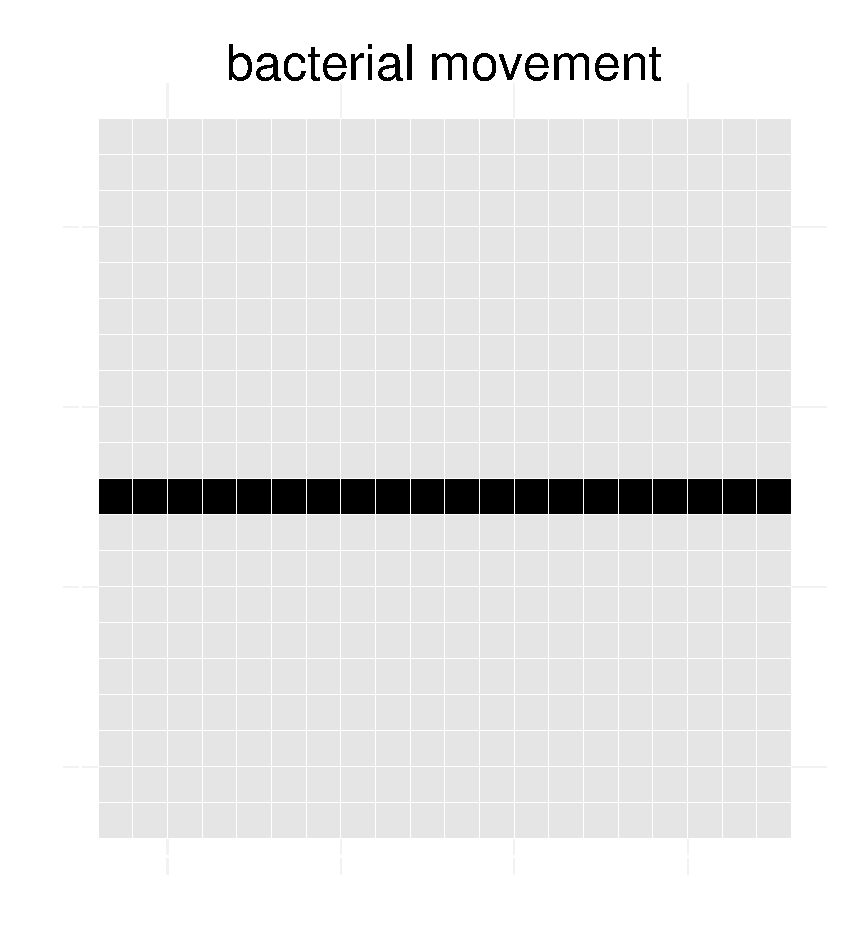
\includegraphics[width=\textwidth]{mov1.pdf}
  \end{minipage}
  \begin{minipage}[t]{0.3\textwidth}
    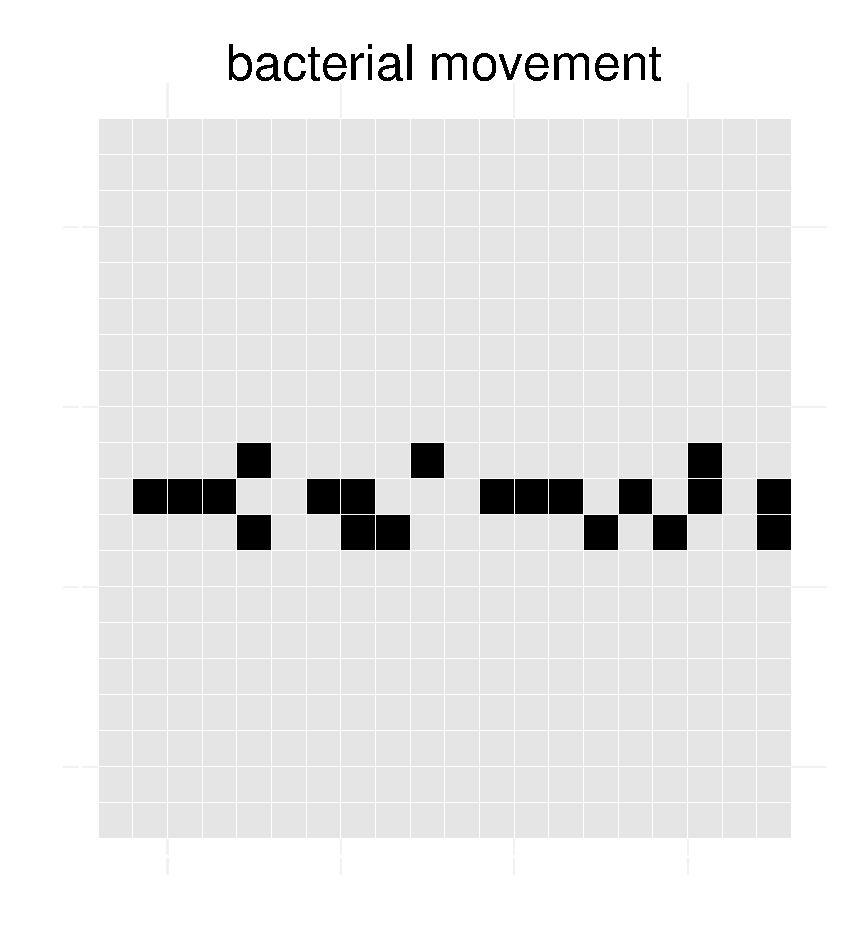
\includegraphics[width=\textwidth]{mov2.pdf}
  \end{minipage}
  \begin{minipage}[t]{0.3\textwidth}
    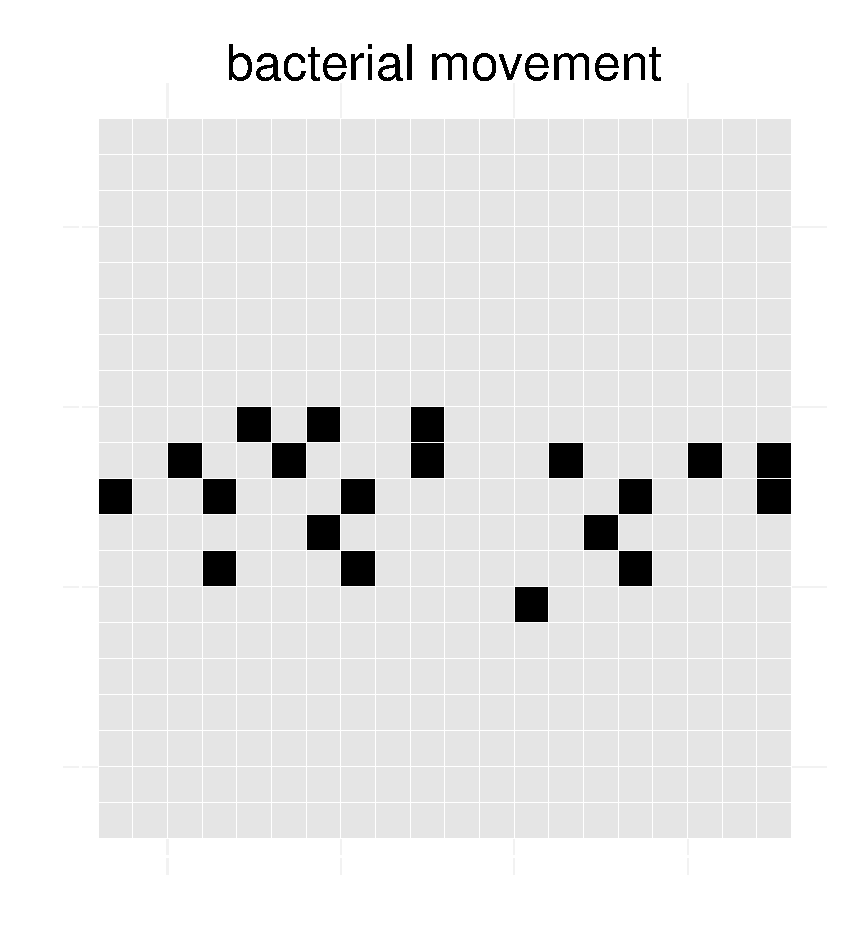
\includegraphics[width=\textwidth]{mov3.pdf}
  \end{minipage}
  \caption{Bacterial movement starting with a line of bacteria in the middle of a $20\times20$ grid. Three different iteration steps are displayed (time step 1, 2 and 5).}
\end{figure}

\begin{figure}[h]
  \centering
  \begin{minipage}[t]{0.3\textwidth}
    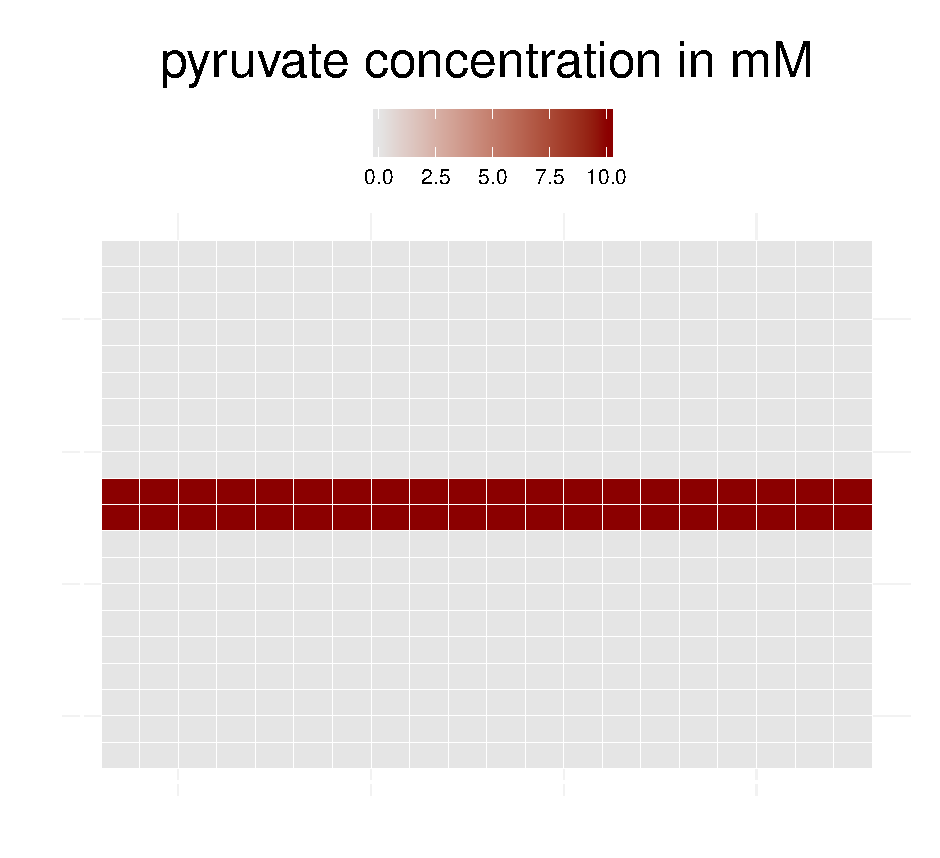
\includegraphics[width=\textwidth]{diff1.pdf}
  \end{minipage}
  \begin{minipage}[t]{0.3\textwidth}
    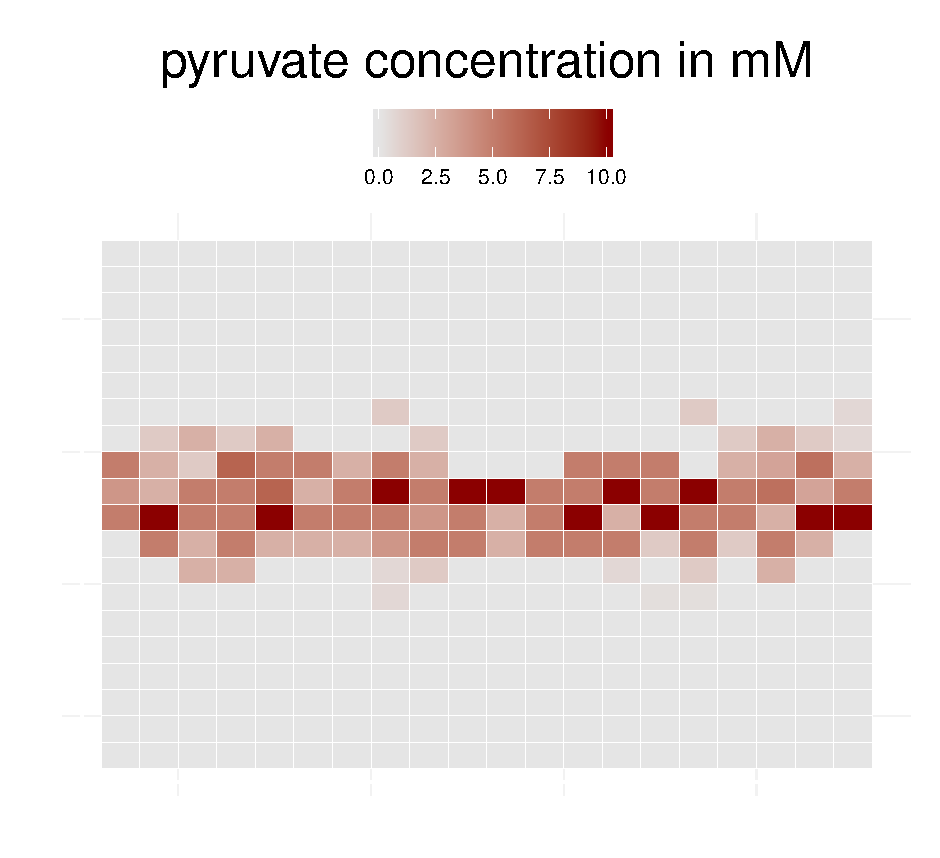
\includegraphics[width=\textwidth]{diff2.pdf}
  \end{minipage}
  \begin{minipage}[t]{0.3\textwidth}
    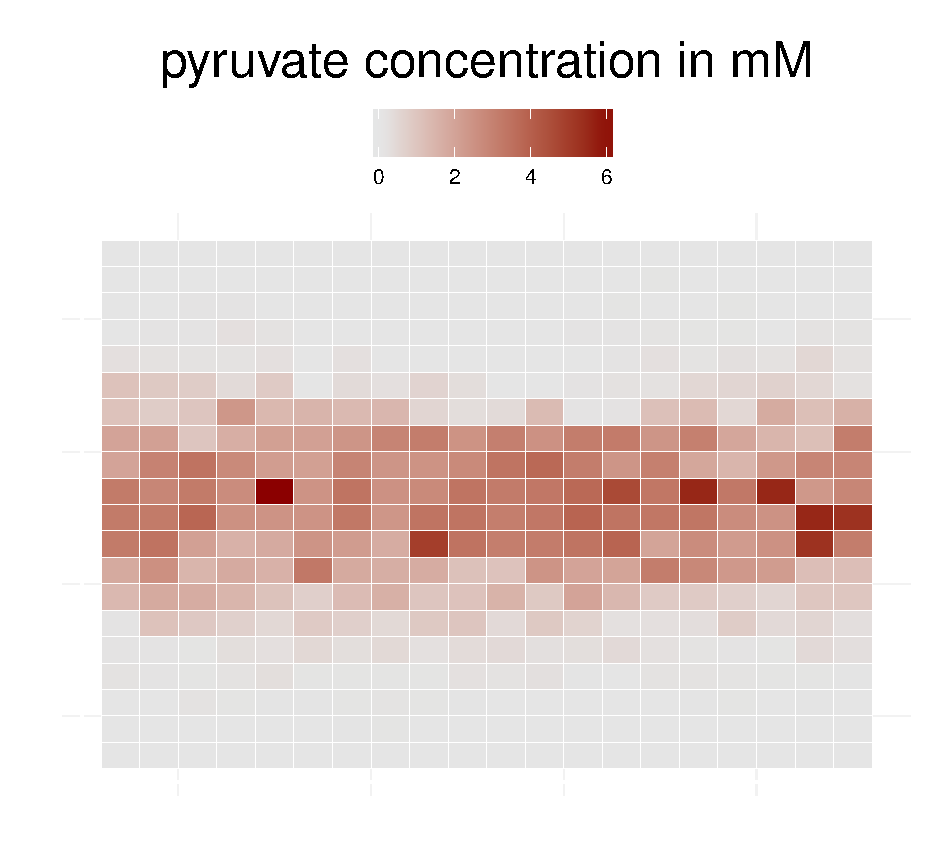
\includegraphics[width=\textwidth]{diff5.pdf}
  \end{minipage}
  \caption{Diffusion starting with 10\;mmol pyruvate in the middle of a $20\times20$ grid. Three different iteration steps are displayed (time step 1, 2 and 5).}
\end{figure}
\subsection{Growth models}
\clearpage
\subsubsection{\textit{Escherichia coli} core}

\begin{figure}[h]
  \centering
  \subfigure[]{
  %\begin{minipage}[t]{0.45\textwidth}
    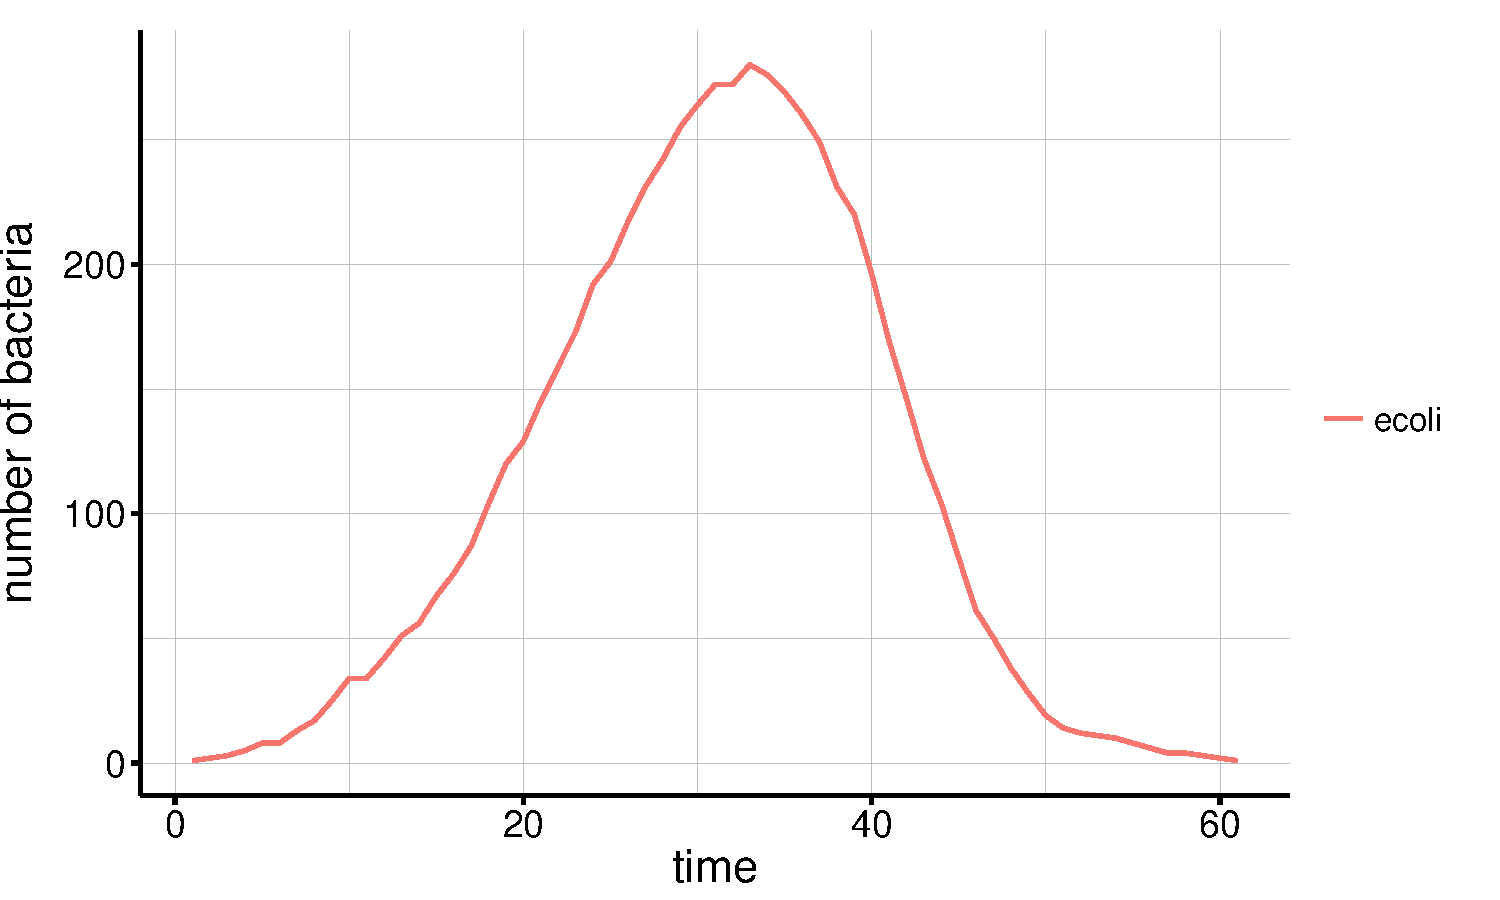
\includegraphics[scale=0.45]{../results/ecoli_20x20_aerob_seed55_growth.pdf}
  %\end{minipage}
  }
  \subfigure[]{
  %\begin{minipage}[t]{0.45\textwidth}
    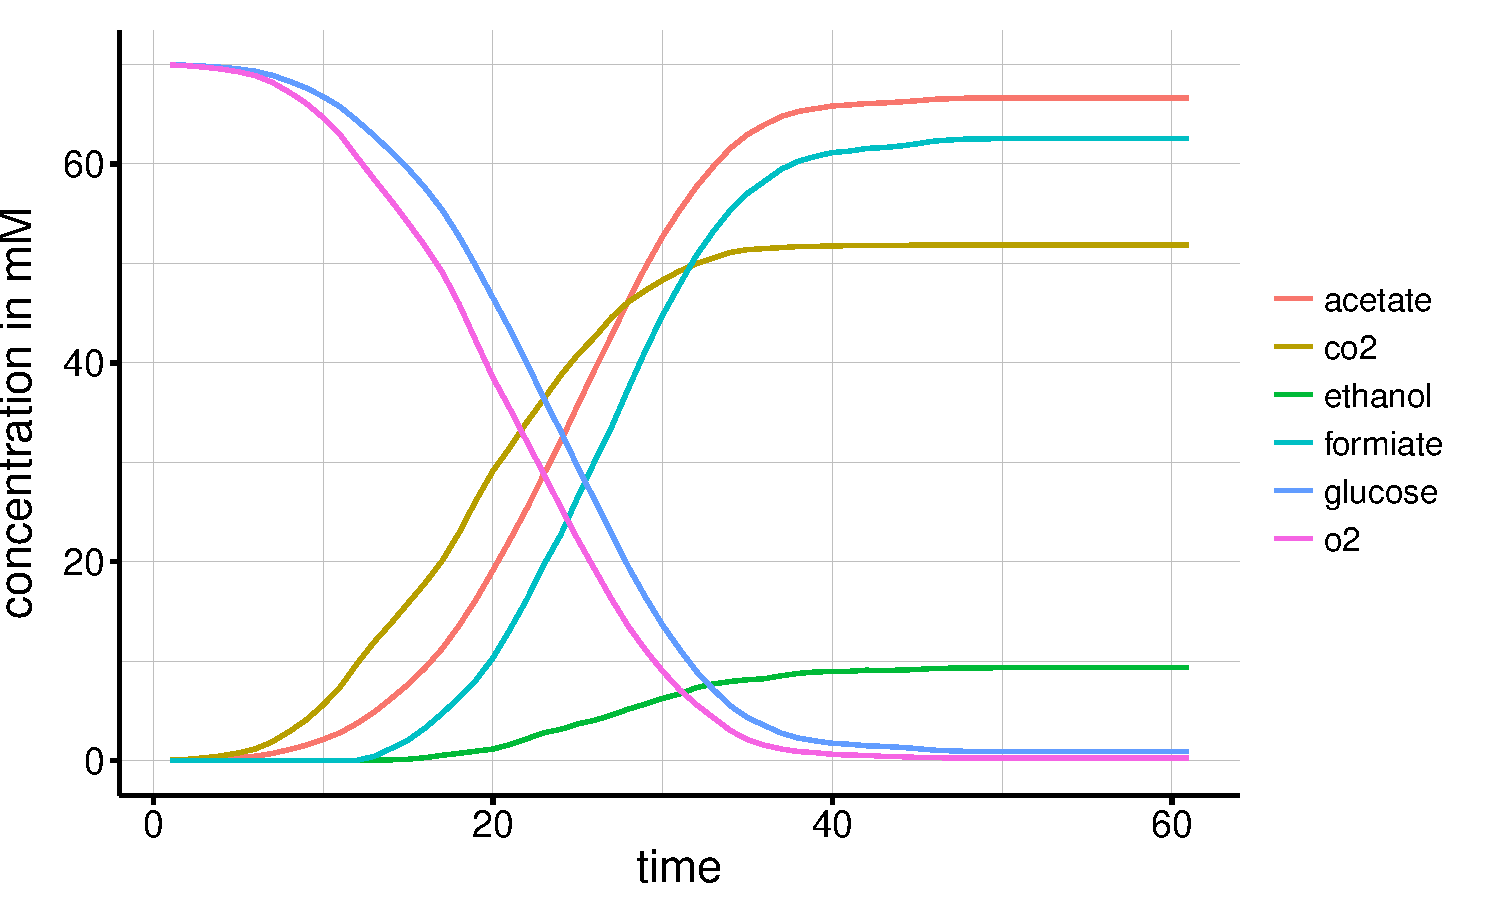
\includegraphics[scale=0.45]{../results/ecoli_20x20_aerob_seed55_subs.pdf}
  %\end{minipage}
  }
  \caption{Population dynamics of the \emph{E. coli} core model on a $20\times20$ grid, with bacterial growth (A) and consumption/production of various metabolites (B). An initial concentration of 70\;mmol per grid cell of glucose and oxygen was added to the environment. The seed of the random number generator was set to 55.}
\end{figure}
\begin{figure}[h]
  \centering
  \subfigure[]{
    \begin{minipage}[t]{0.3\textwidth}
    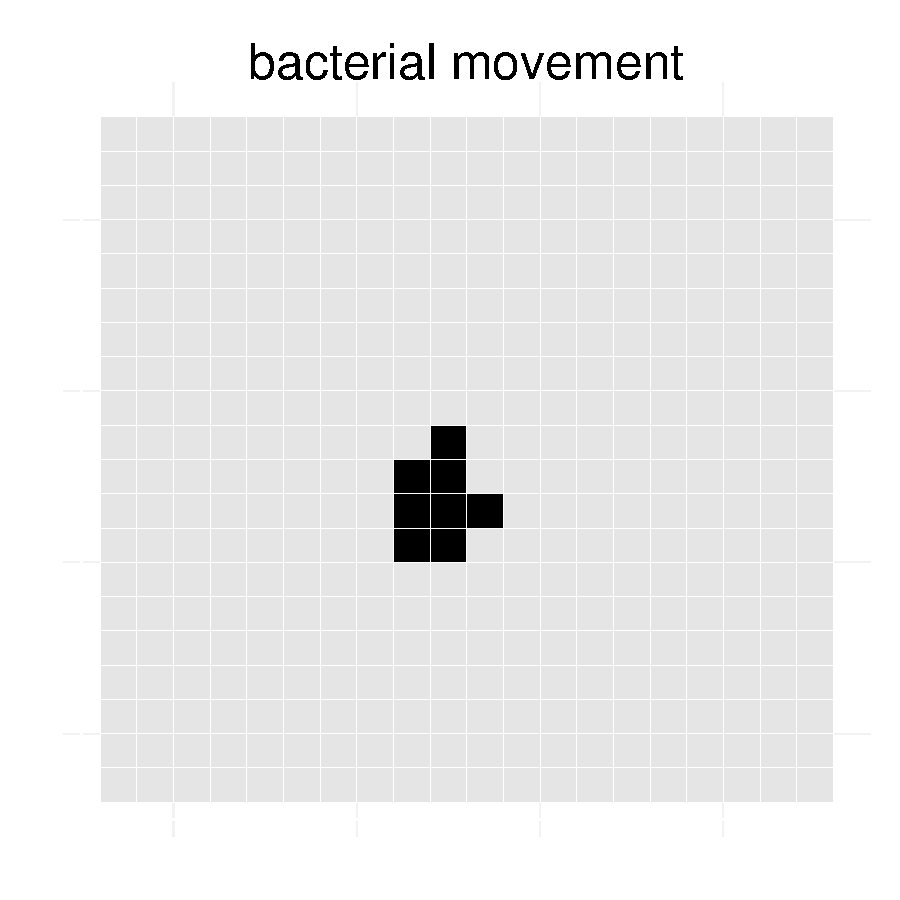
\includegraphics[width=\textwidth]{../results/ecoli_20x20_aerob_seed55_bac5.pdf}
  \end{minipage}
  \begin{minipage}[t]{0.3\textwidth}
    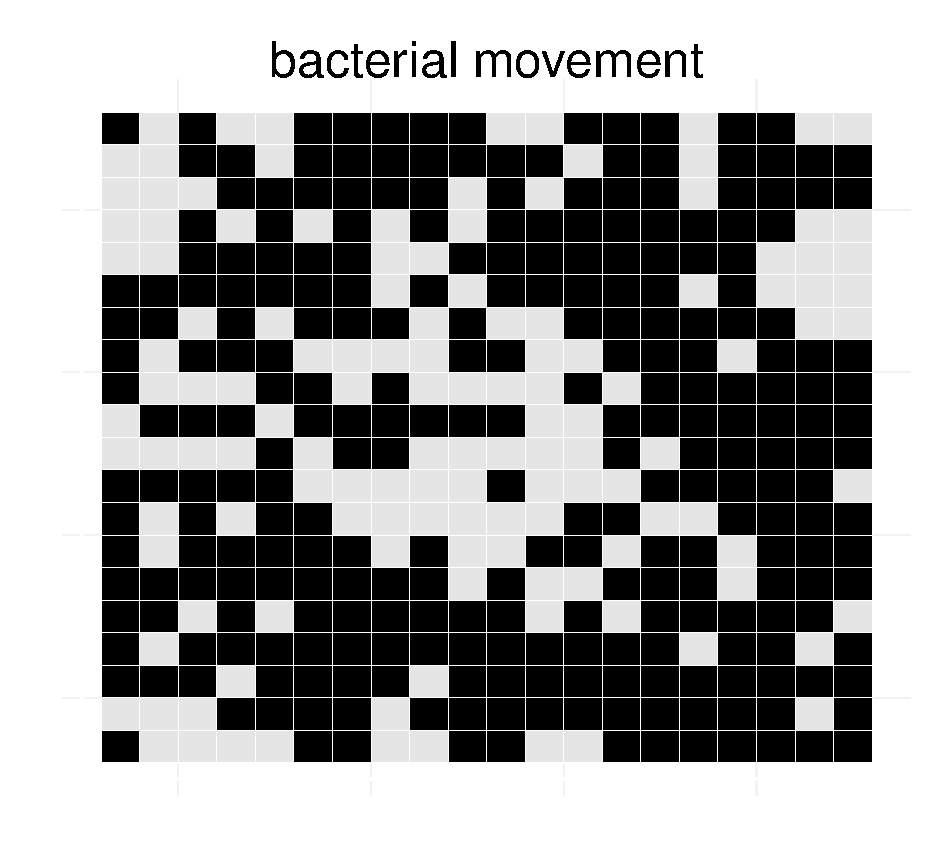
\includegraphics[width=\textwidth]{../results/ecoli_20x20_aerob_seed55_bac35.pdf}
  \end{minipage}
  \begin{minipage}[t]{0.3\textwidth}
    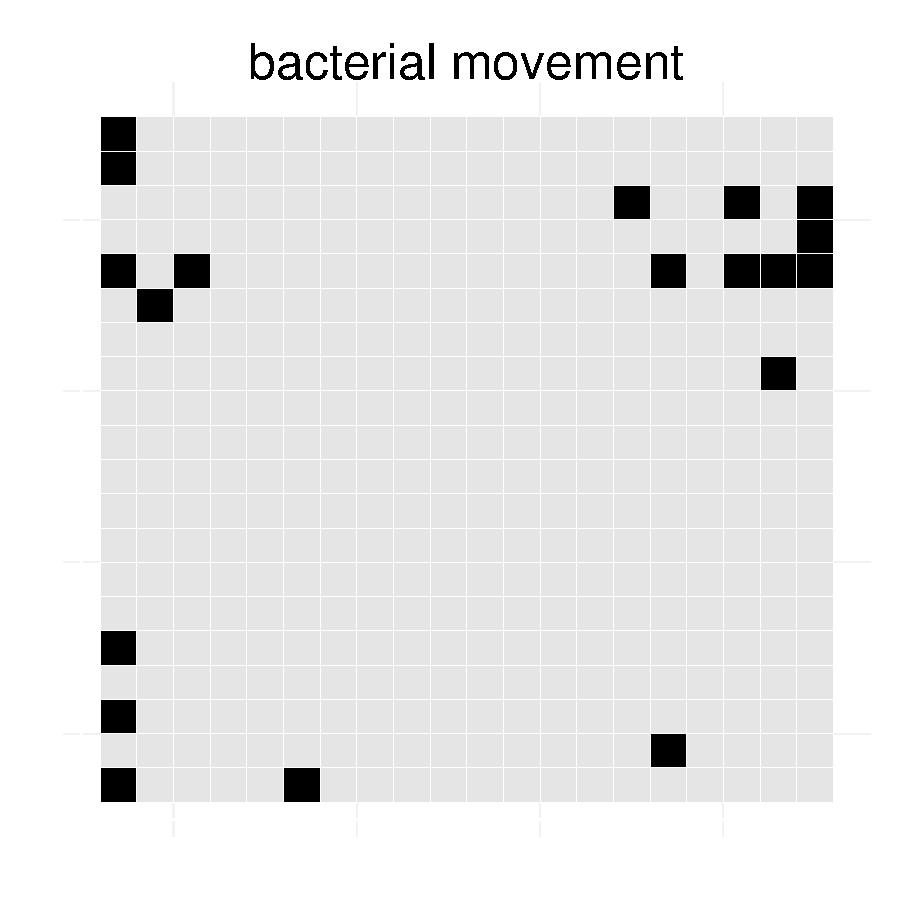
\includegraphics[width=\textwidth]{../results/ecoli_20x20_aerob_seed55_bac50.pdf}
  \end{minipage}
  }
  \subfigure[]{
  \begin{minipage}[t]{0.3\textwidth}
    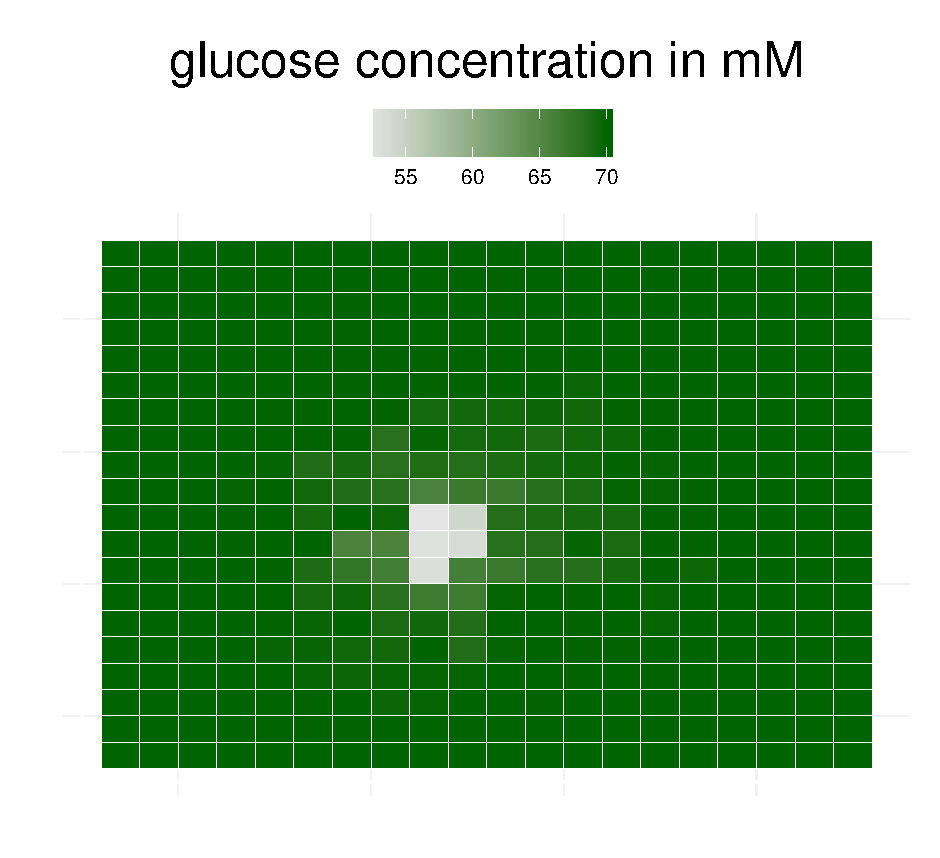
\includegraphics[width=\textwidth]{../results/ecoli_20x20_aerob_seed55_gluc5.pdf}
  \end{minipage}
  \begin{minipage}[t]{0.3\textwidth}
    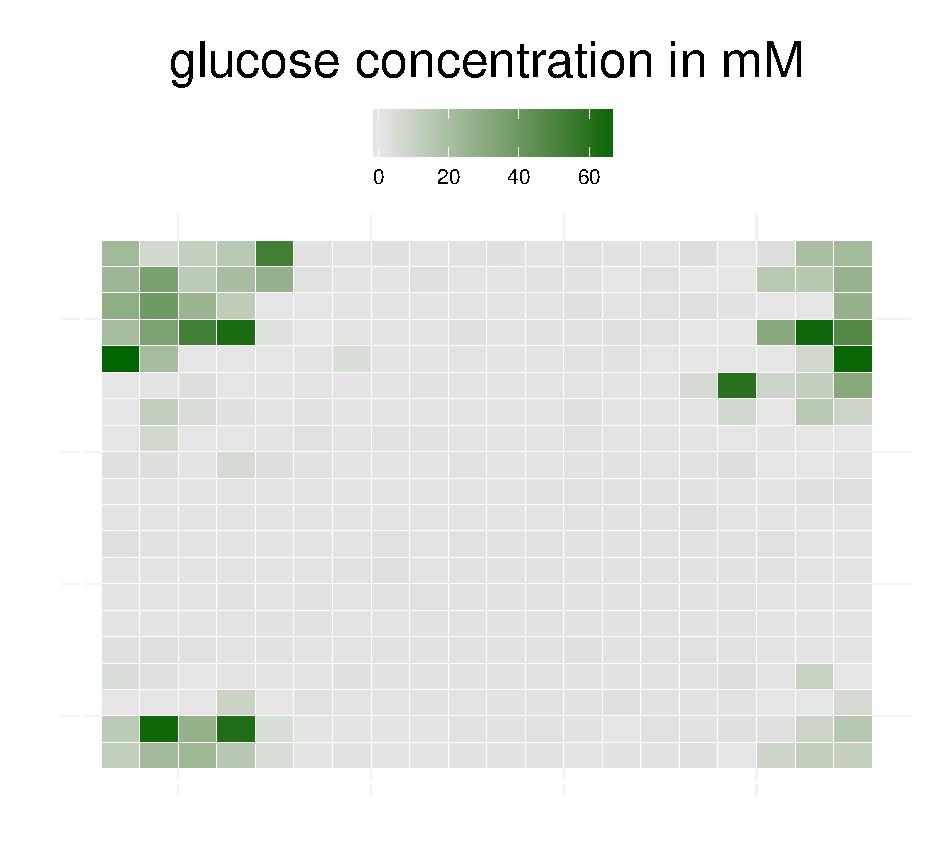
\includegraphics[width=\textwidth]{../results/ecoli_20x20_aerob_seed55_gluc35.pdf}
  \end{minipage}
  \begin{minipage}[t]{0.3\textwidth}
    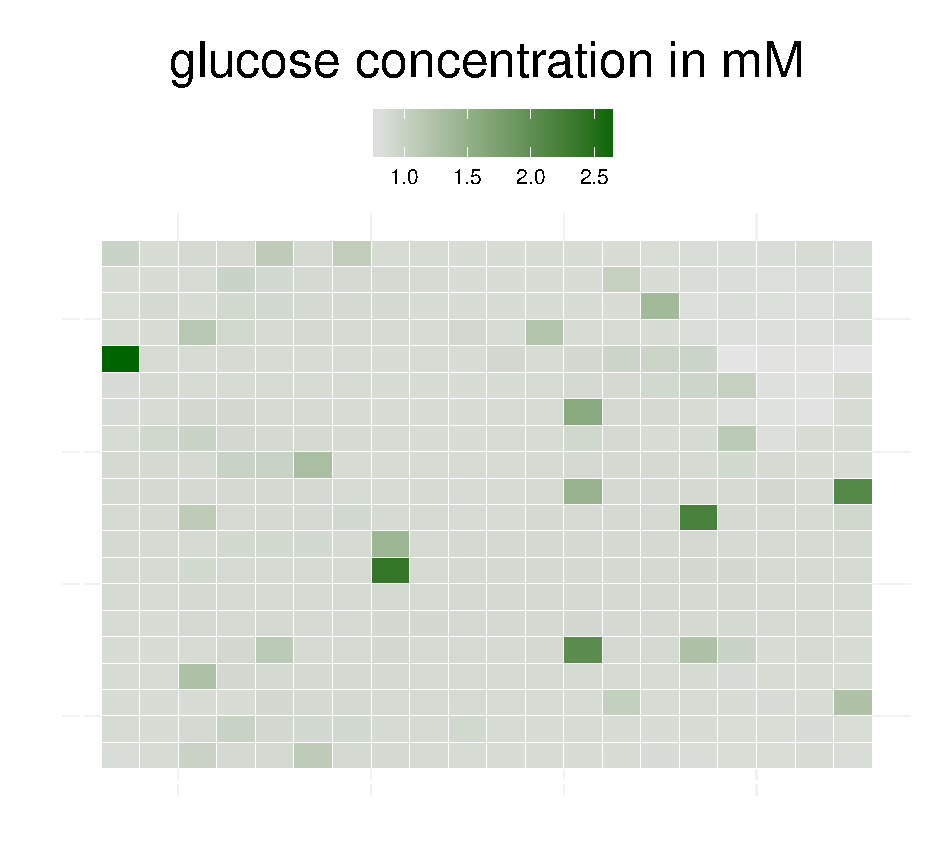
\includegraphics[width=\textwidth]{../results/ecoli_20x20_aerob_seed55_gluc50.pdf}
  \end{minipage}
  }
  \subfigure[]{
  \begin{minipage}[t]{0.3\textwidth}
    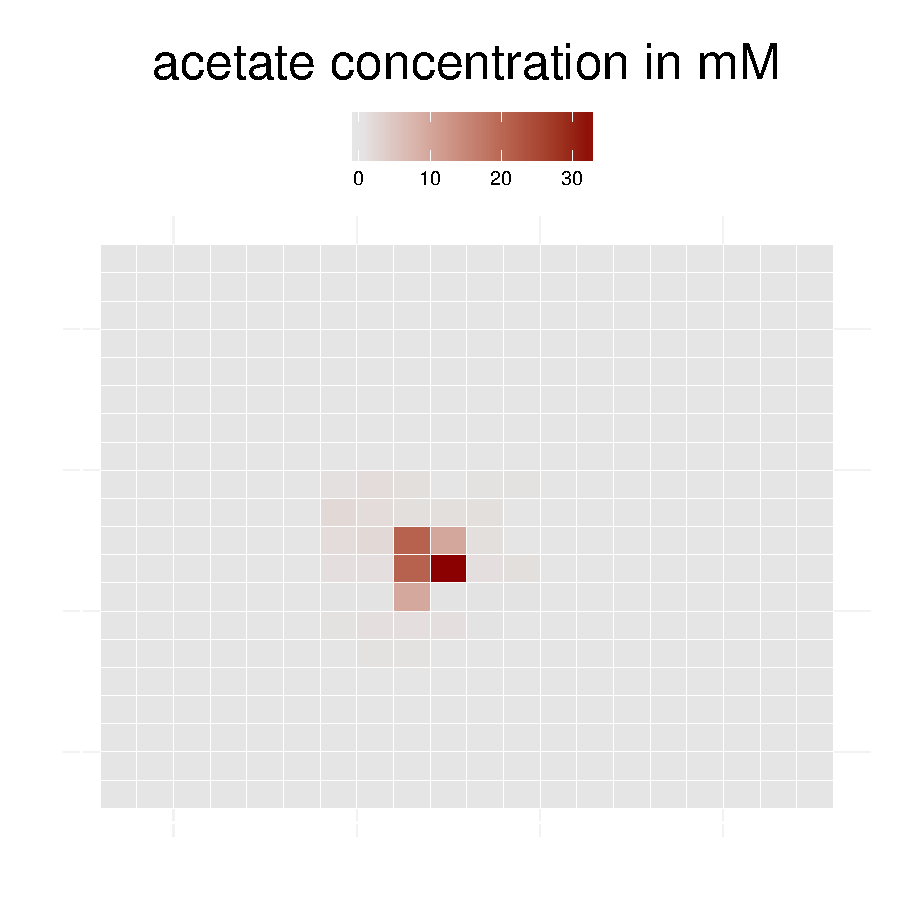
\includegraphics[width=\textwidth]{../results/ecoli_20x20_aerob_seed55_ace5.pdf}
  \end{minipage}
  \begin{minipage}[t]{0.3\textwidth}
    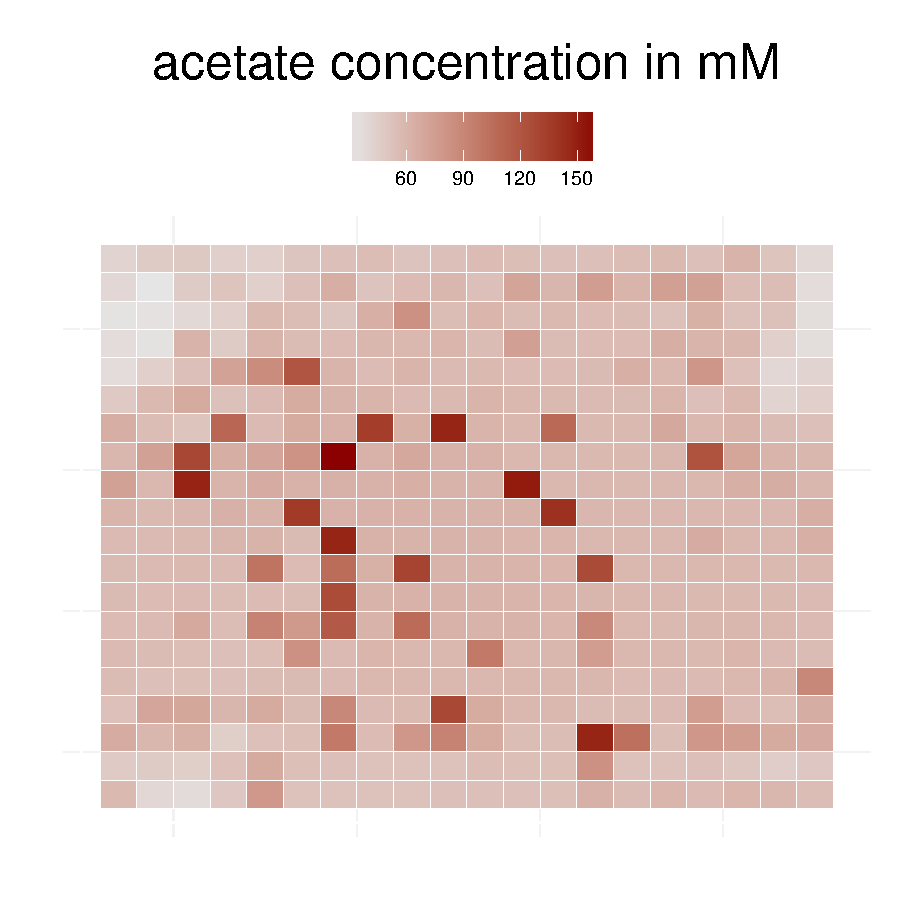
\includegraphics[width=\textwidth]{../results/ecoli_20x20_aerob_seed55_ace35.pdf}
  \end{minipage}
  \begin{minipage}[t]{0.3\textwidth}
    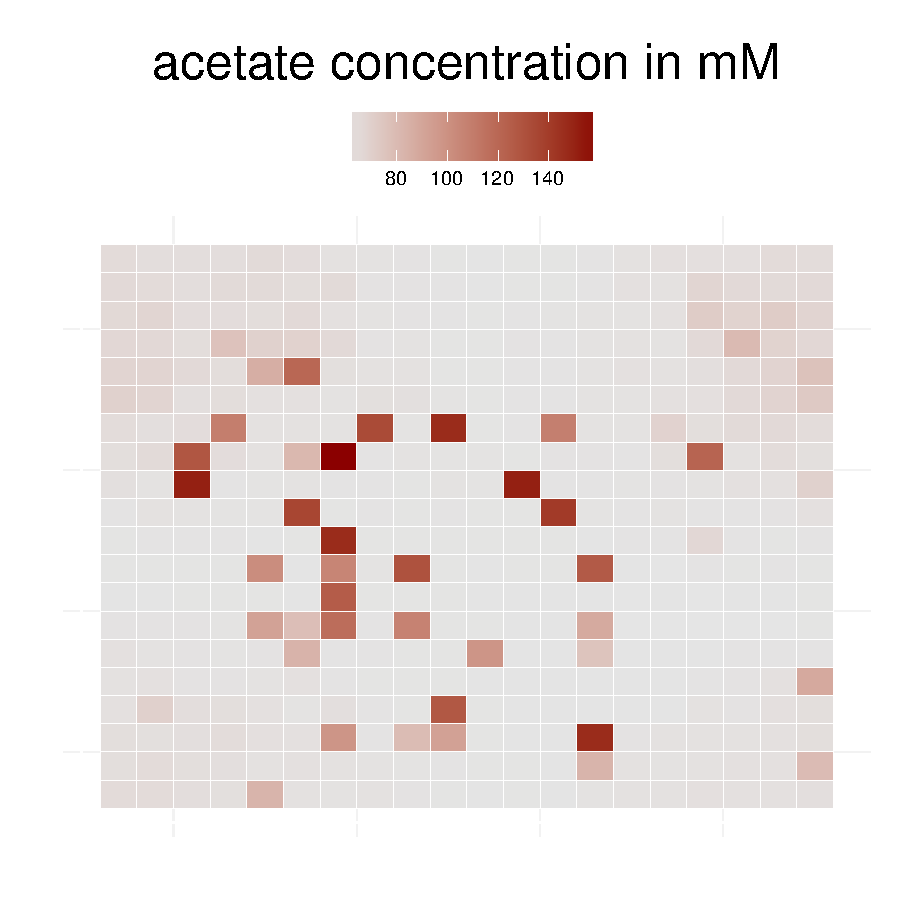
\includegraphics[width=\textwidth]{../results/ecoli_20x20_aerob_seed55_ace50.pdf}
  \end{minipage}
  }
  \subfigure[]{
  \begin{minipage}[t]{0.3\textwidth}
    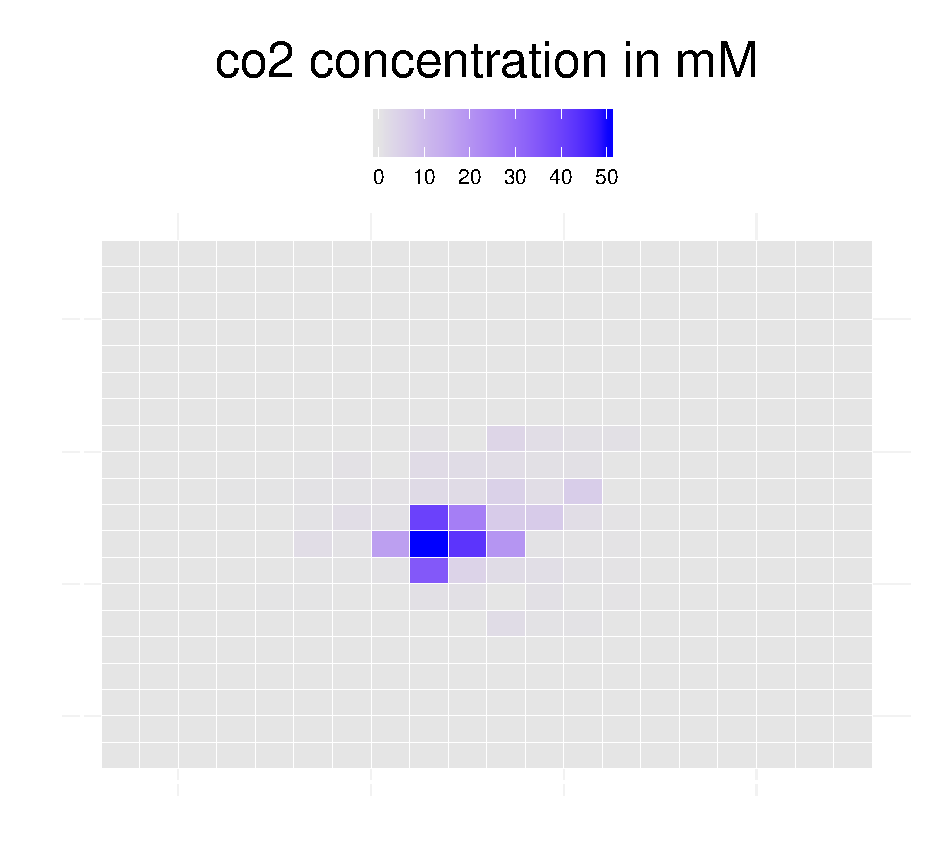
\includegraphics[width=\textwidth]{../results/ecoli_20x20_aerob_seed55_co25.pdf}
  \end{minipage}
  \begin{minipage}[t]{0.3\textwidth}
    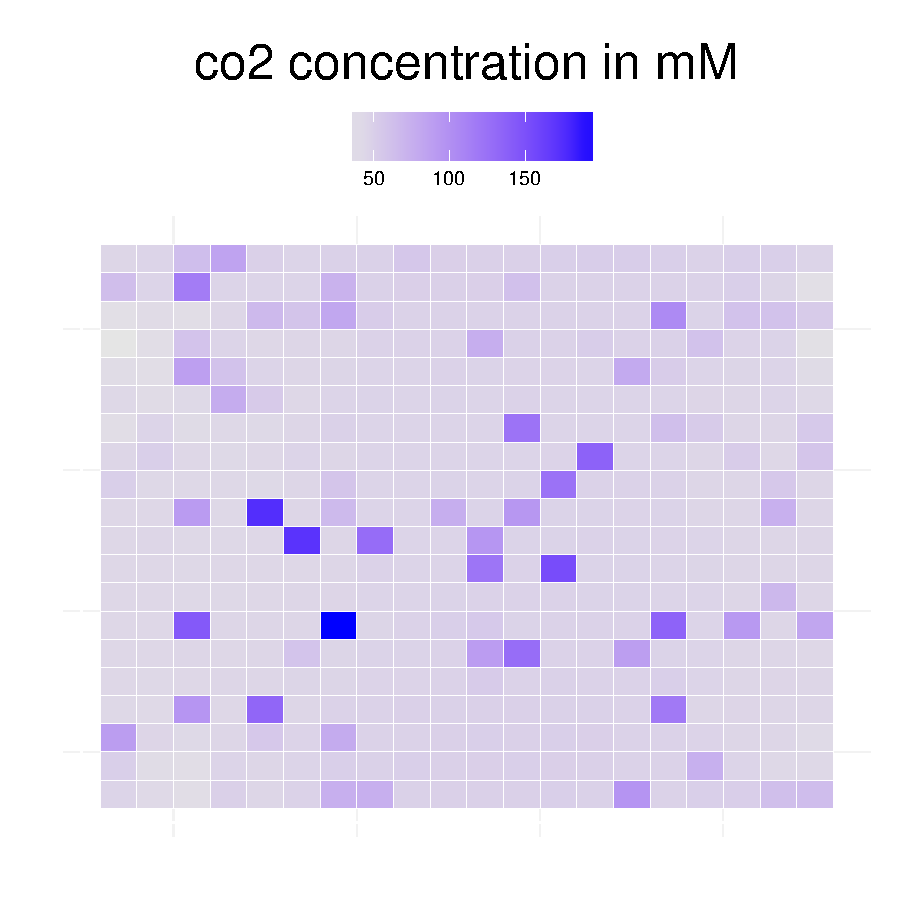
\includegraphics[width=\textwidth]{../results/ecoli_20x20_aerob_seed55_co235.pdf}
  \end{minipage}
  \begin{minipage}[t]{0.3\textwidth}
    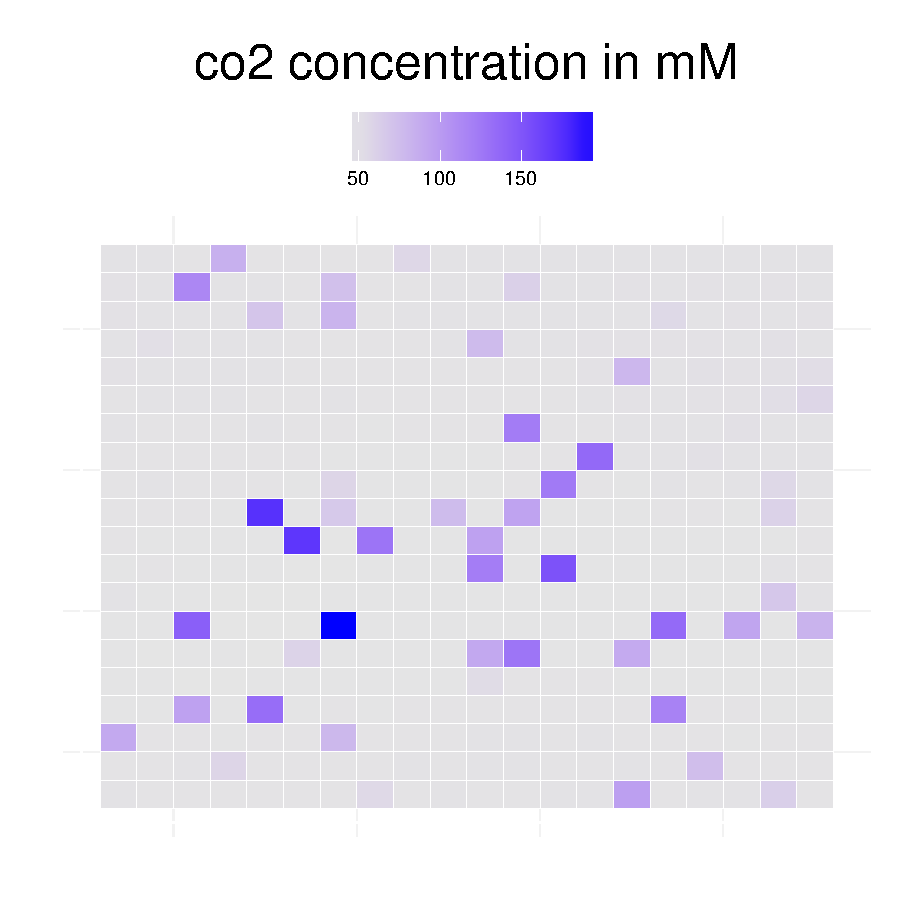
\includegraphics[width=\textwidth]{../results/ecoli_20x20_aerob_seed55_co250.pdf}
  \end{minipage}
  }
  \caption{Population dynamics of the \emph{E. coli} core model on a $20\times20$ grid, with bacterial movement (A) and concentrations of glucose (B), acetate (C) and CO$_2$ (D) (of time step 5, 35 and 50). The seed of the random number generator was set to 55.}
\end{figure}

\subsubsection{\textit{Escherichia coli}}

\begin{figure}[h]
  \centering
    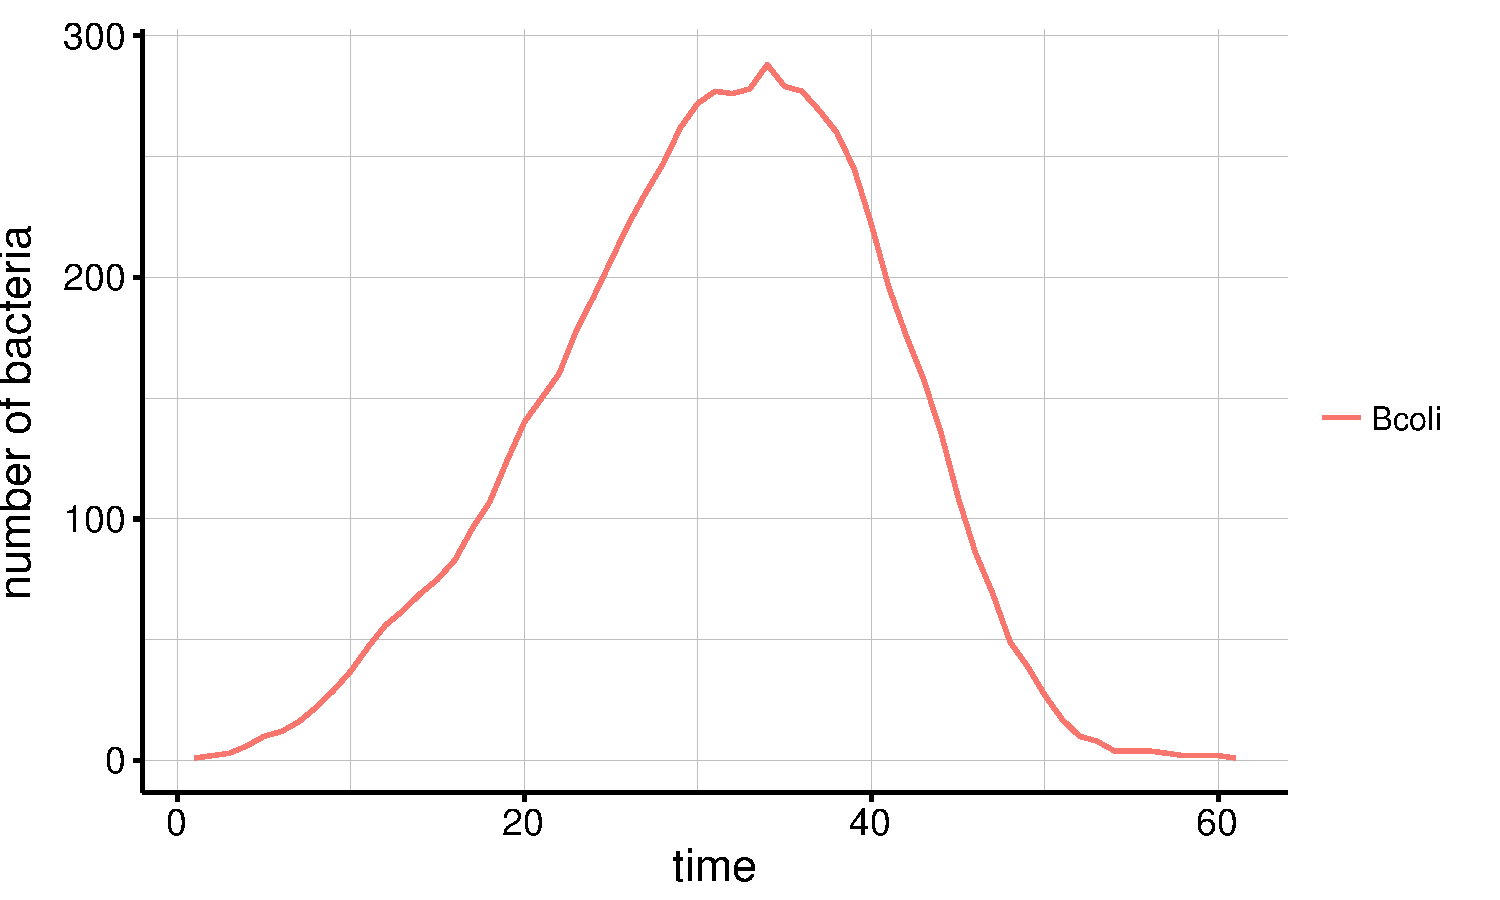
\includegraphics[scale=0.45]{../results/Bcoli_20x20_seed176_growth.pdf}
    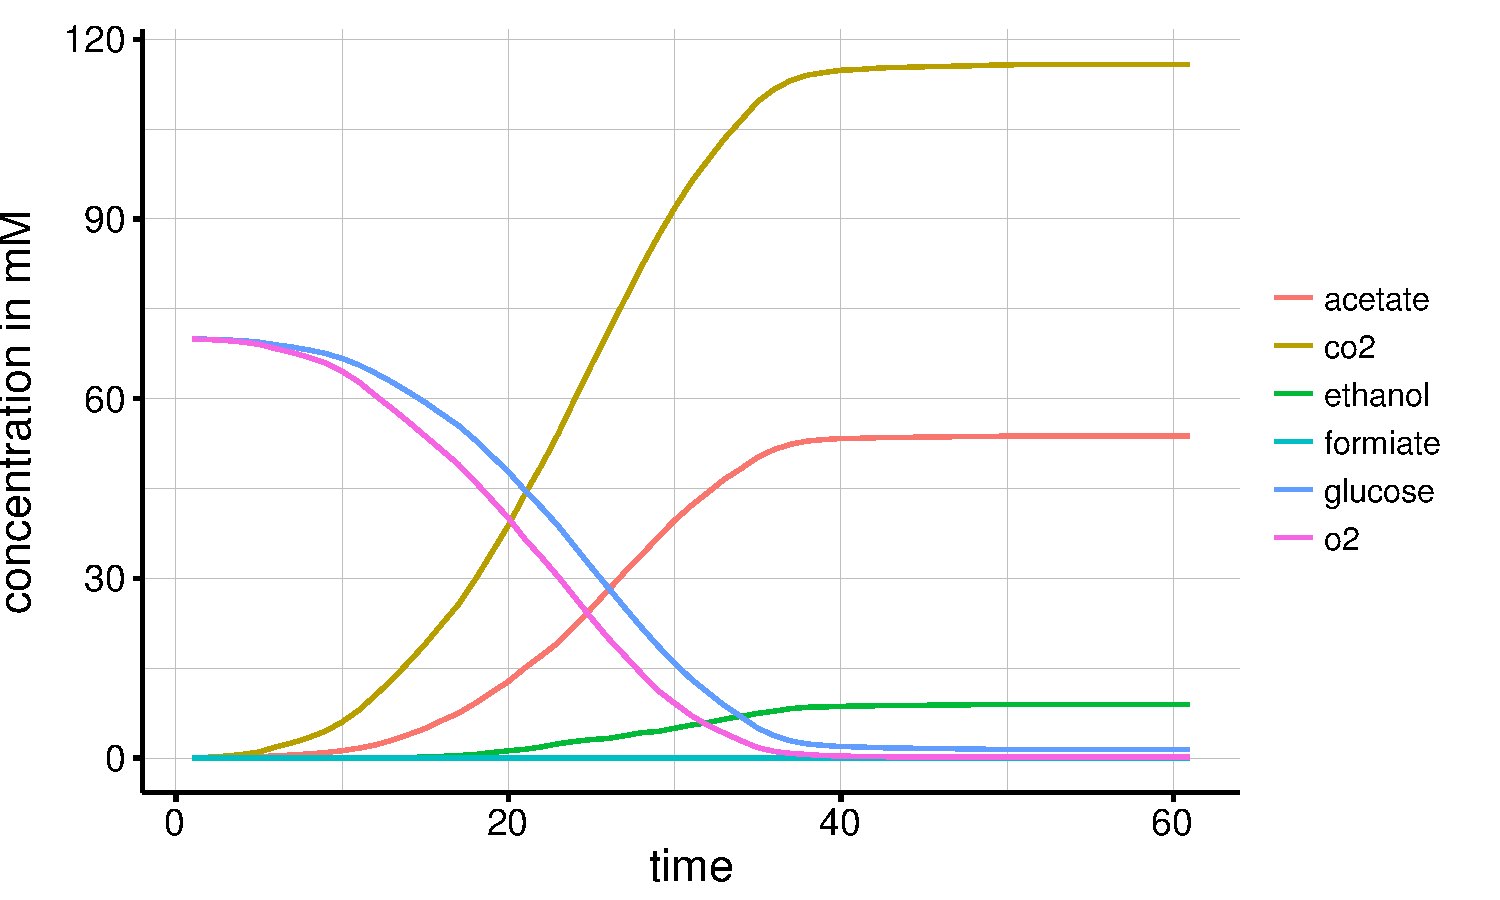
\includegraphics[scale=0.45]{../results/Bcoli_20x20_seed176_subs.pdf}
  \caption{Population dynamics of the \emph{E. coli} model on a $20\times20$ grid, with bacterial growth (A) and consumption/production of various metabolites (B). An initial concentration of 70\;mmol per grid cell of glucose and oxygen was added to the environment. The seed of the random number generator was set to 176.}
\end{figure}
\begin{figure}[h]
  \centering
  \subfigure[]{
    \begin{minipage}[t]{0.3\textwidth}
    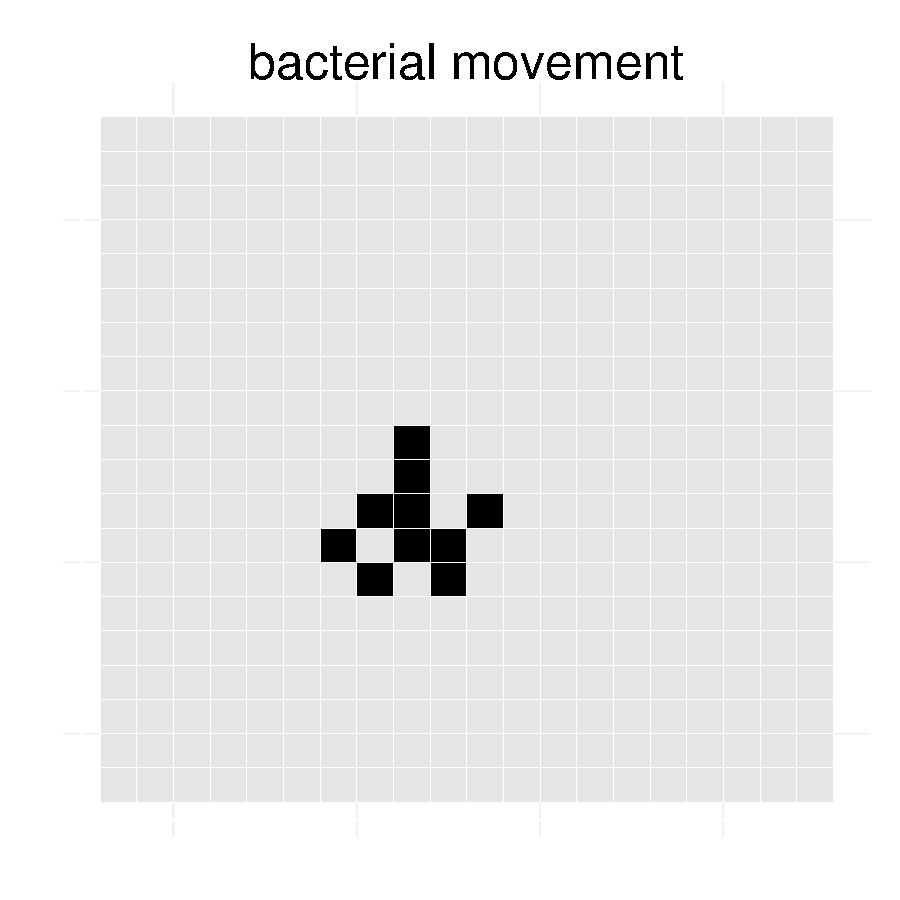
\includegraphics[width=\textwidth]{../results/Bcoli_20x20_seed176_bac5.pdf}
  \end{minipage}
  \begin{minipage}[t]{0.3\textwidth}
    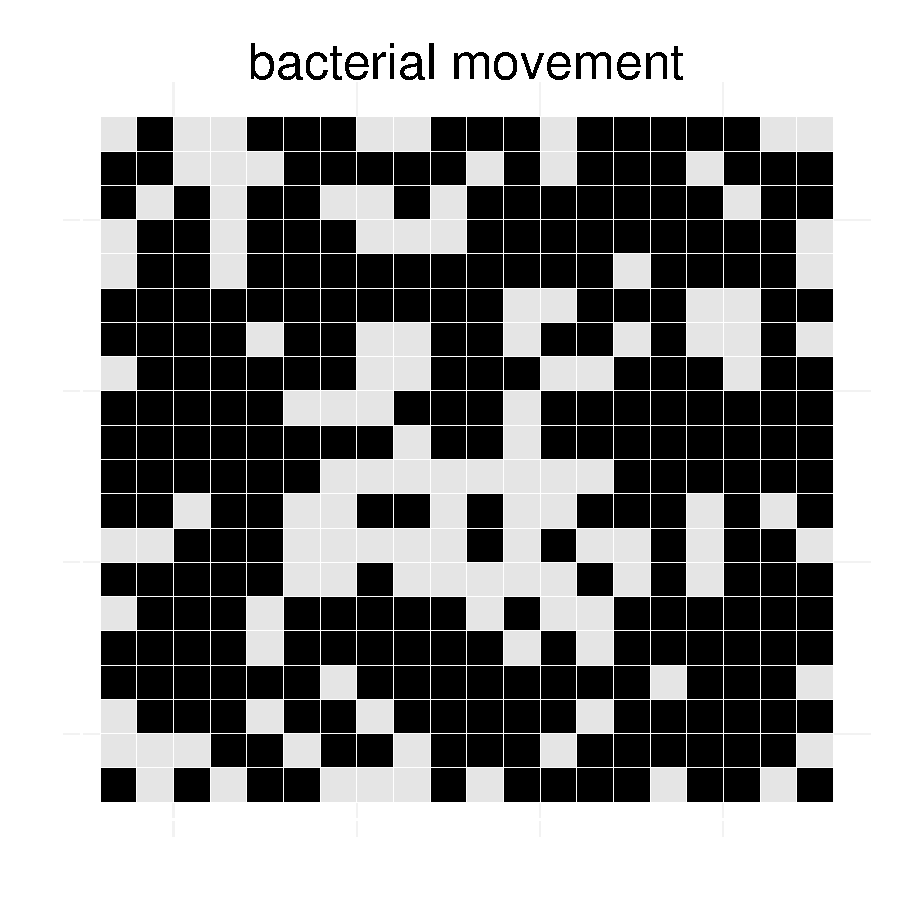
\includegraphics[width=\textwidth]{../results/Bcoli_20x20_seed176_bac35.pdf}
  \end{minipage}
  \begin{minipage}[t]{0.3\textwidth}
    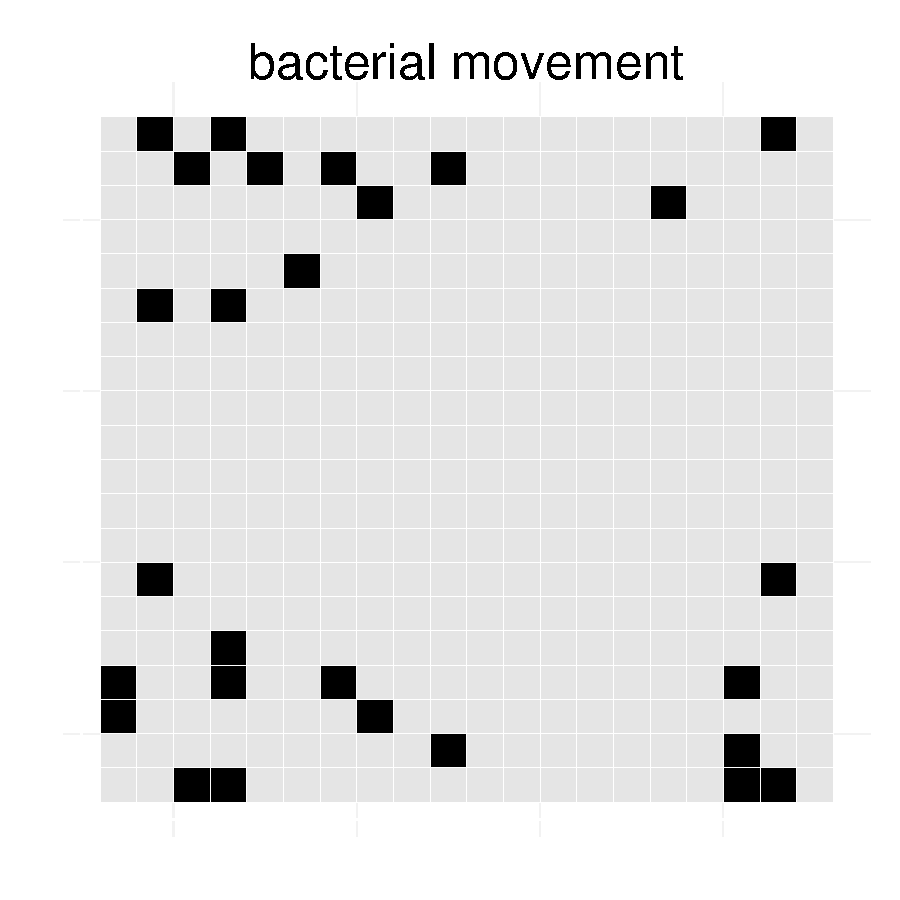
\includegraphics[width=\textwidth]{../results/Bcoli_20x20_seed176_bac50.pdf}
  \end{minipage}
  }
  \subfigure[]{
  \begin{minipage}[t]{0.3\textwidth}
    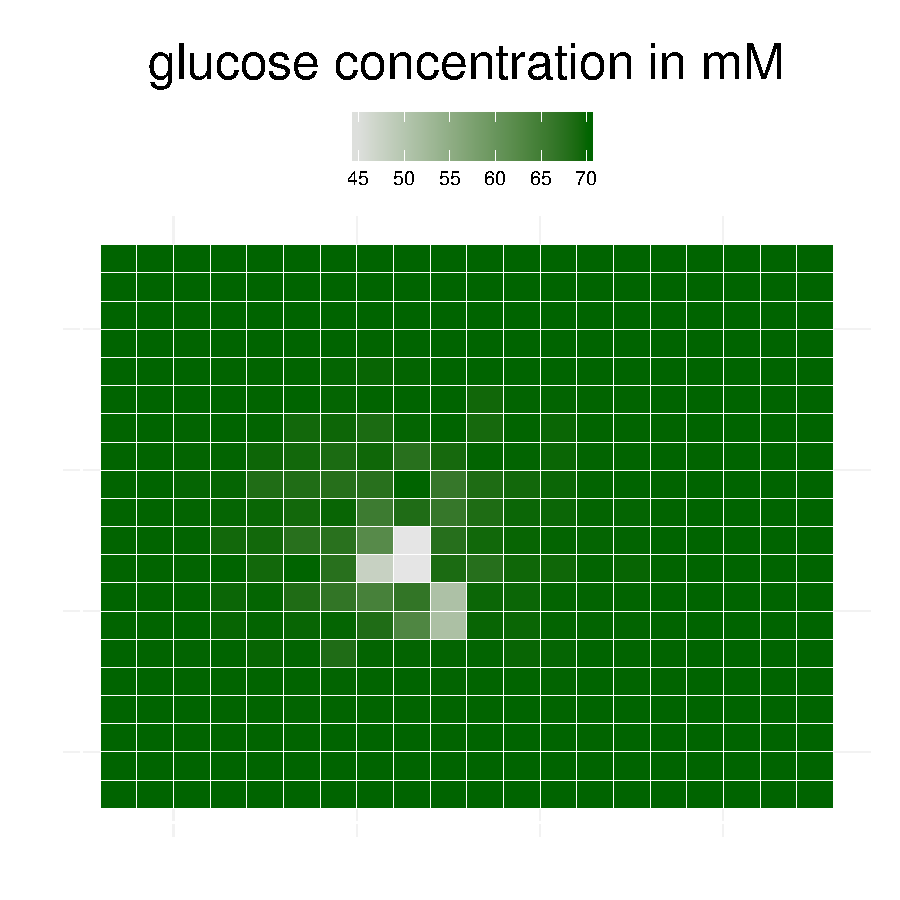
\includegraphics[width=\textwidth]{../results/Bcoli_20x20_seed176_gluc5.pdf}
  \end{minipage}
  \begin{minipage}[t]{0.3\textwidth}
    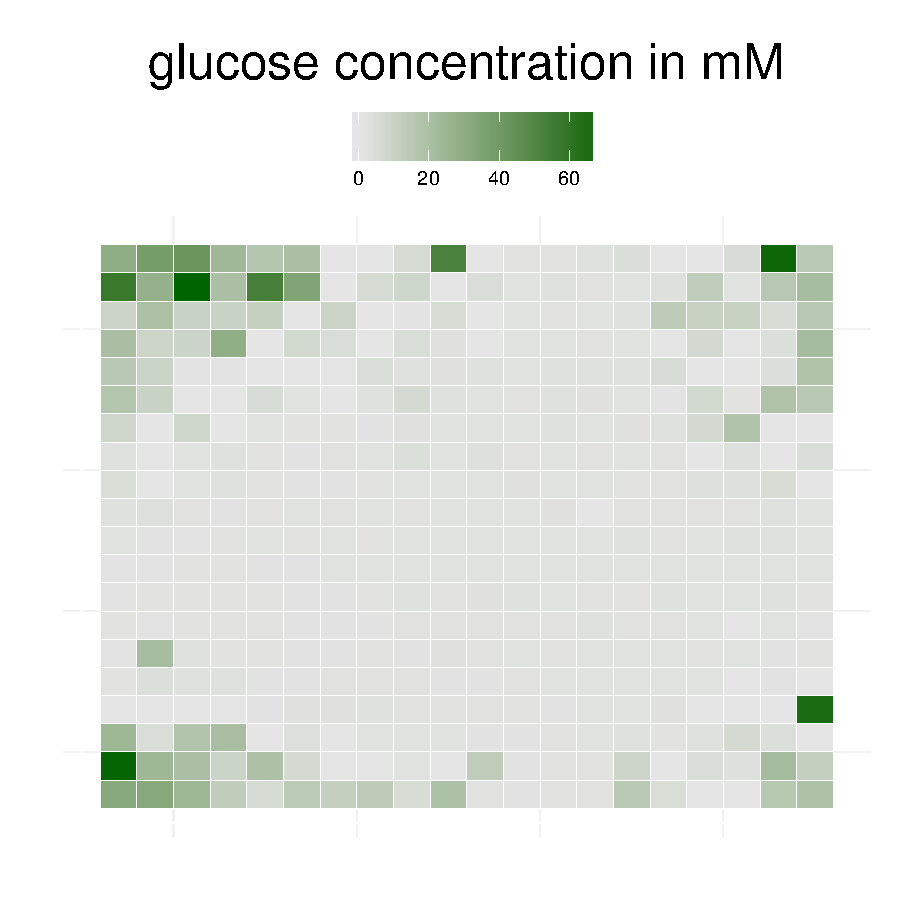
\includegraphics[width=\textwidth]{../results/Bcoli_20x20_seed176_gluc35.pdf}
  \end{minipage}
  \begin{minipage}[t]{0.3\textwidth}
    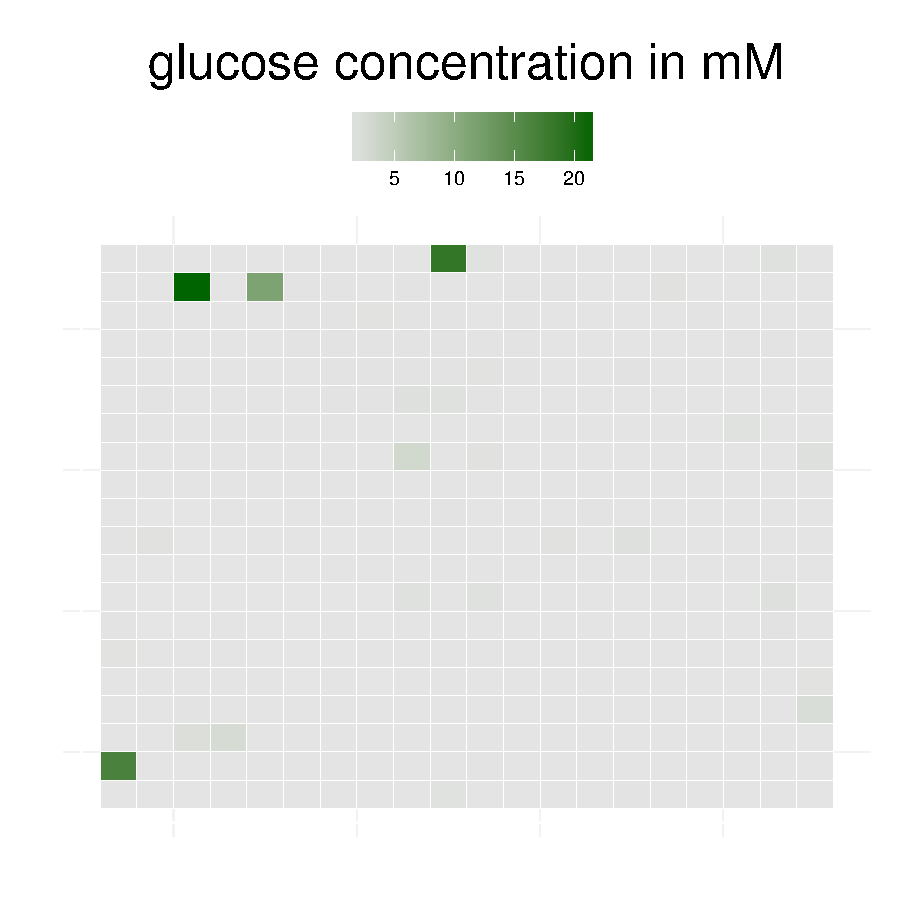
\includegraphics[width=\textwidth]{../results/Bcoli_20x20_seed176_gluc50.pdf}
  \end{minipage}
  }
  \subfigure[]{
  \begin{minipage}[t]{0.3\textwidth}
    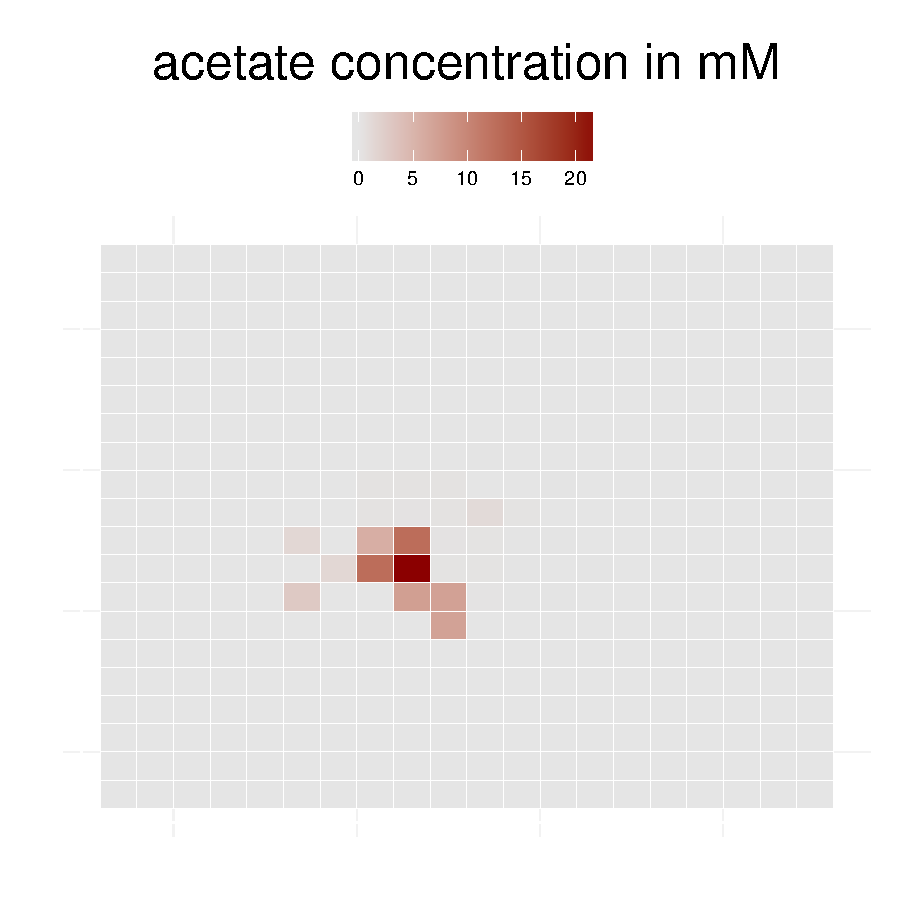
\includegraphics[width=\textwidth]{../results/Bcoli_20x20_seed176_ace5.pdf}
  \end{minipage}
  \begin{minipage}[t]{0.3\textwidth}
    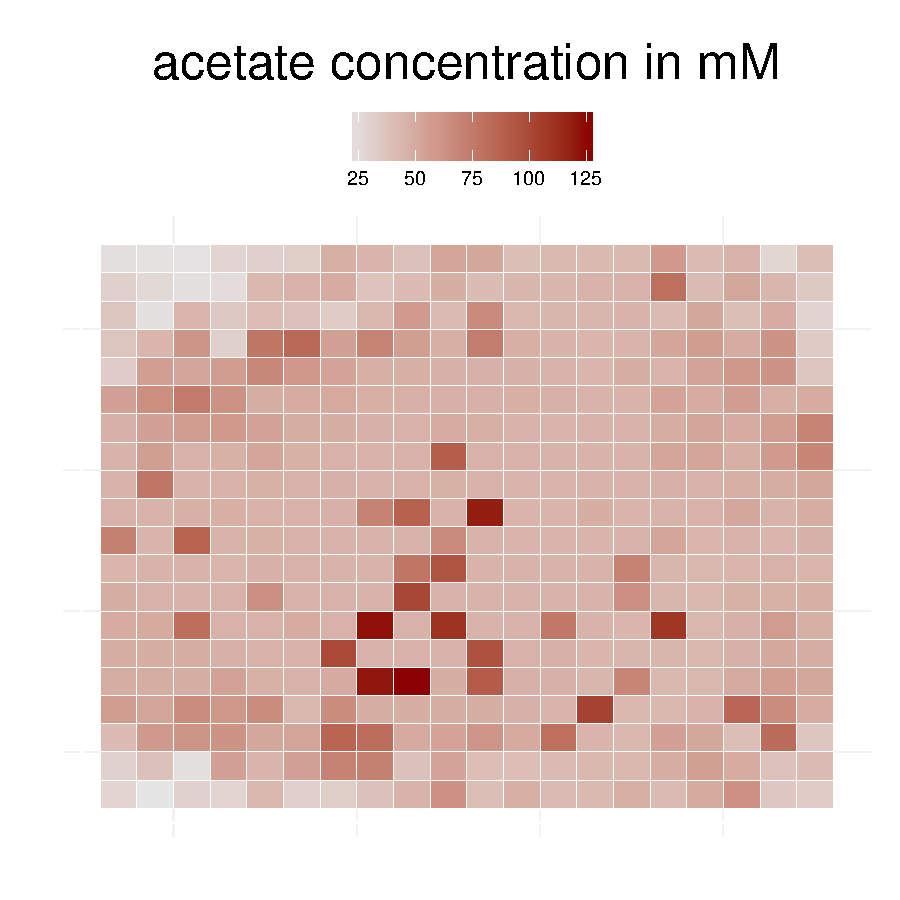
\includegraphics[width=\textwidth]{../results/Bcoli_20x20_seed176_ace35.pdf}
  \end{minipage}
  \begin{minipage}[t]{0.3\textwidth}
    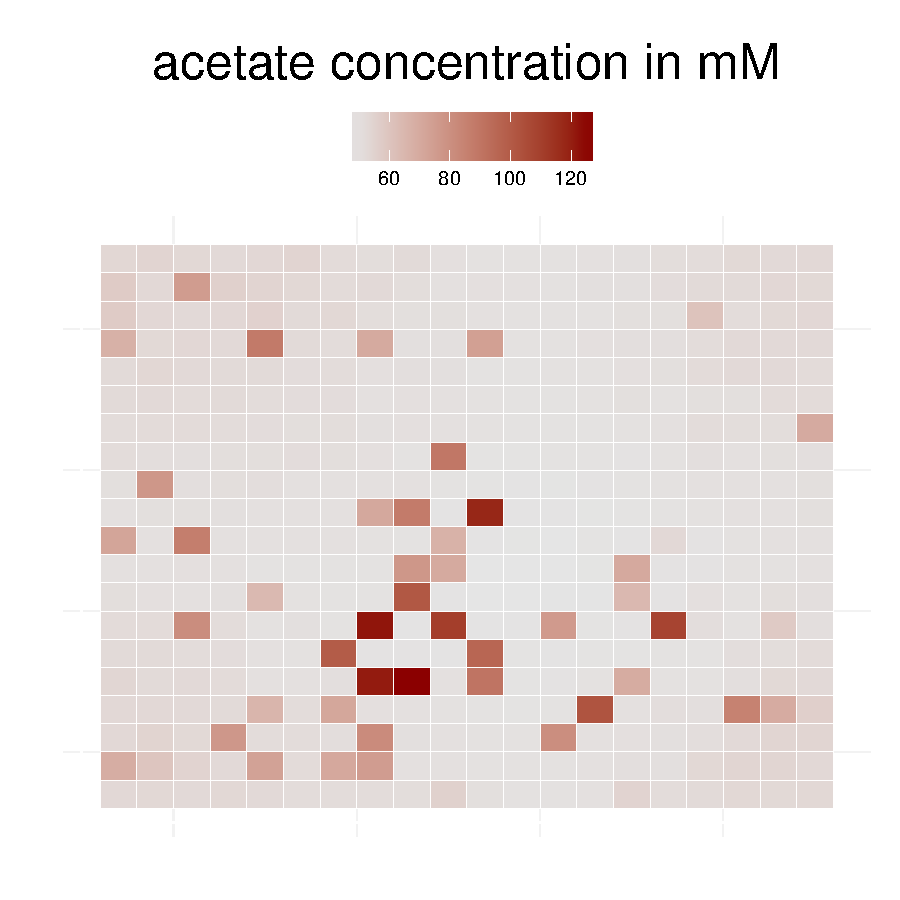
\includegraphics[width=\textwidth]{../results/Bcoli_20x20_seed176_ace50.pdf}
  \end{minipage}
  }
  \subfigure[]{
  \begin{minipage}[t]{0.3\textwidth}
    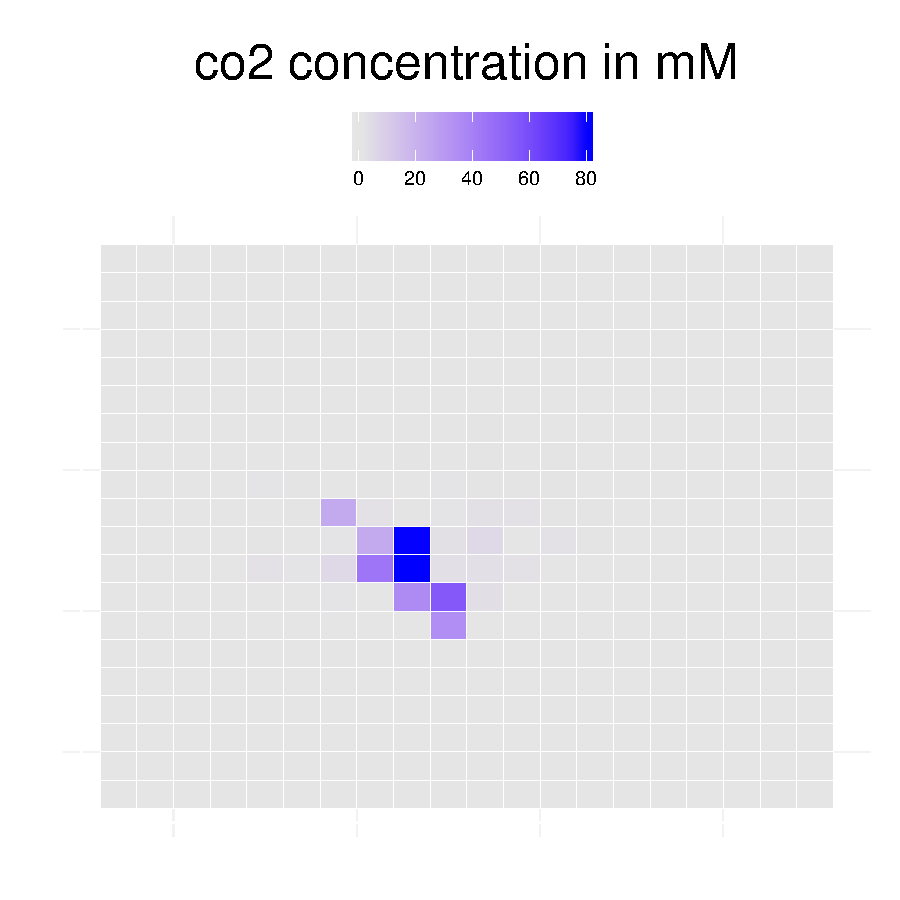
\includegraphics[width=\textwidth]{../results/Bcoli_20x20_seed176_co25.pdf}
  \end{minipage}
  \begin{minipage}[t]{0.3\textwidth}
    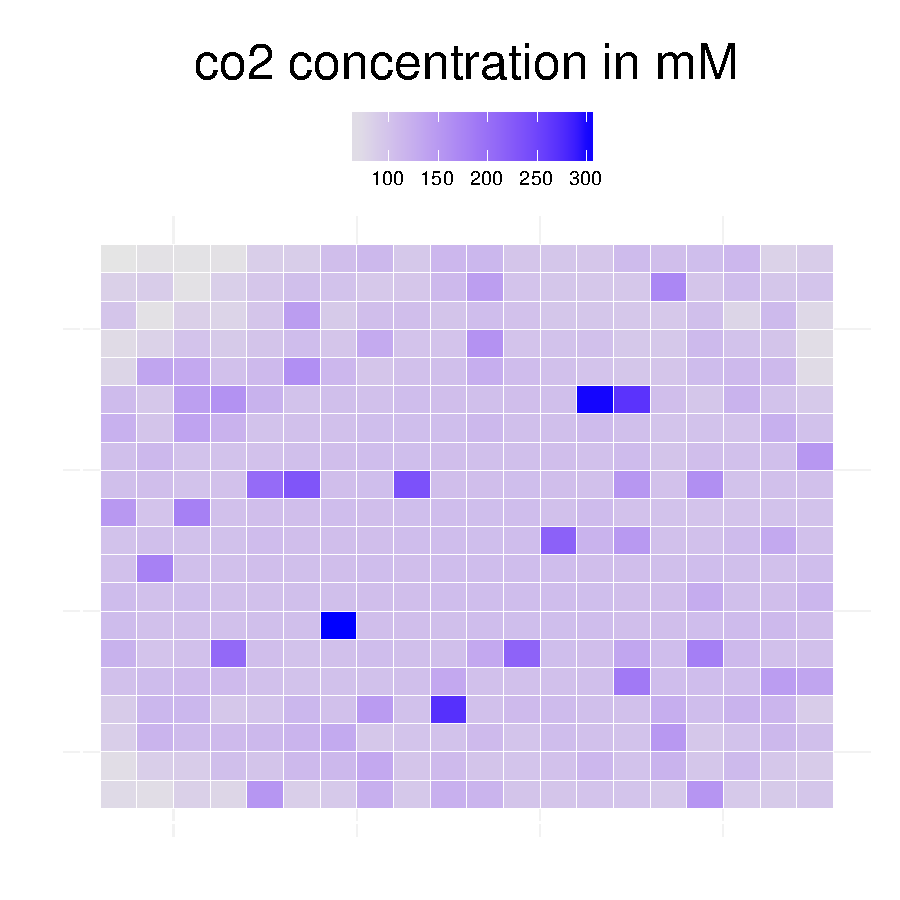
\includegraphics[width=\textwidth]{../results/Bcoli_20x20_seed176_co235.pdf}
  \end{minipage}
  \begin{minipage}[t]{0.3\textwidth}
    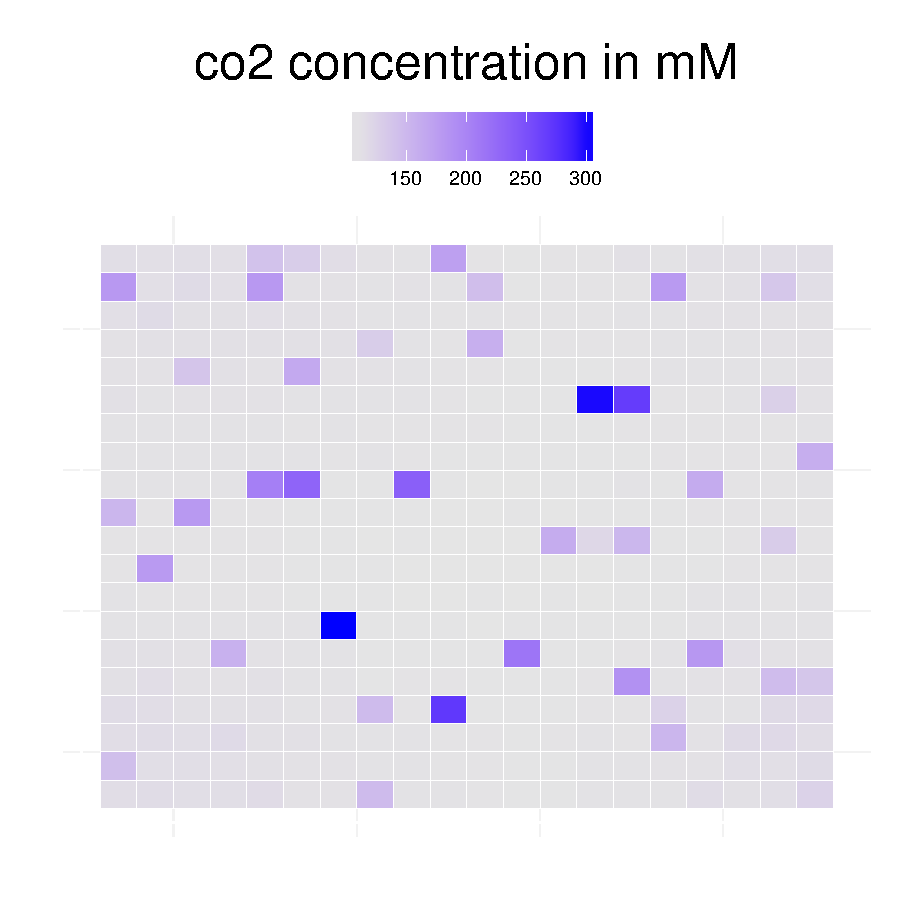
\includegraphics[width=\textwidth]{../results/Bcoli_20x20_seed176_co250.pdf}
  \end{minipage}
  }
  \caption{Population dynamics of the \emph{E. coli} model on a $20\times20$ grid, with bacterial movement (A) and concentrations of glucose (B), acetate (C) and CO$_2$ (D) (of time step 5, 35 and 50). The seed of the random number generator was set to 176.}
\end{figure}

\subsubsection{\textit{Methanosarcina barkeri}}

\begin{figure}[h]
  \centering
    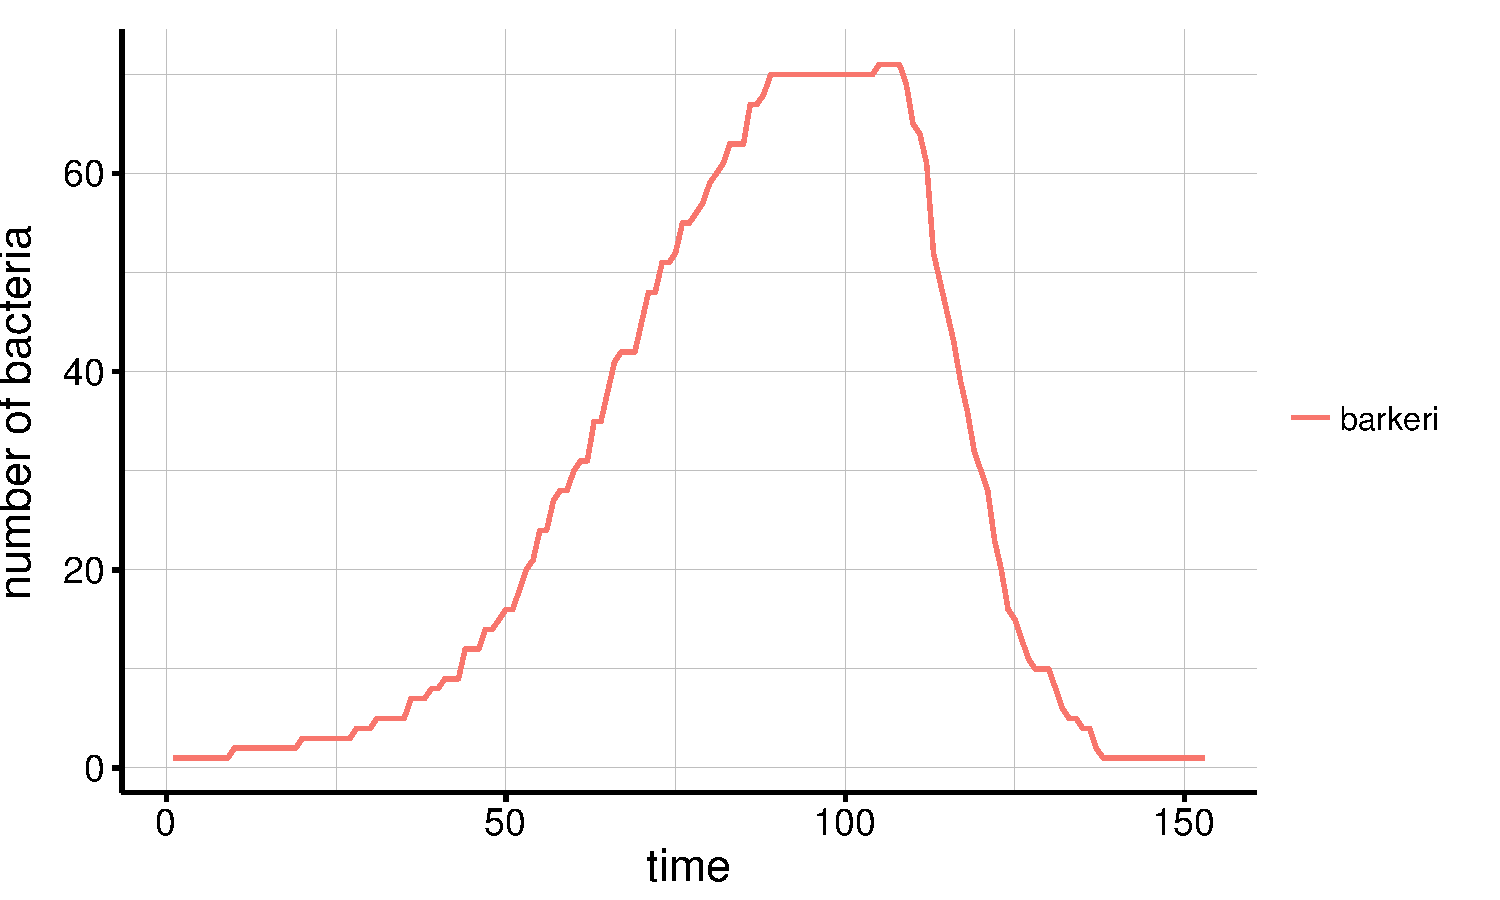
\includegraphics[scale=0.45]{../results/barkeri_20x20_seed9659_growth.pdf}
    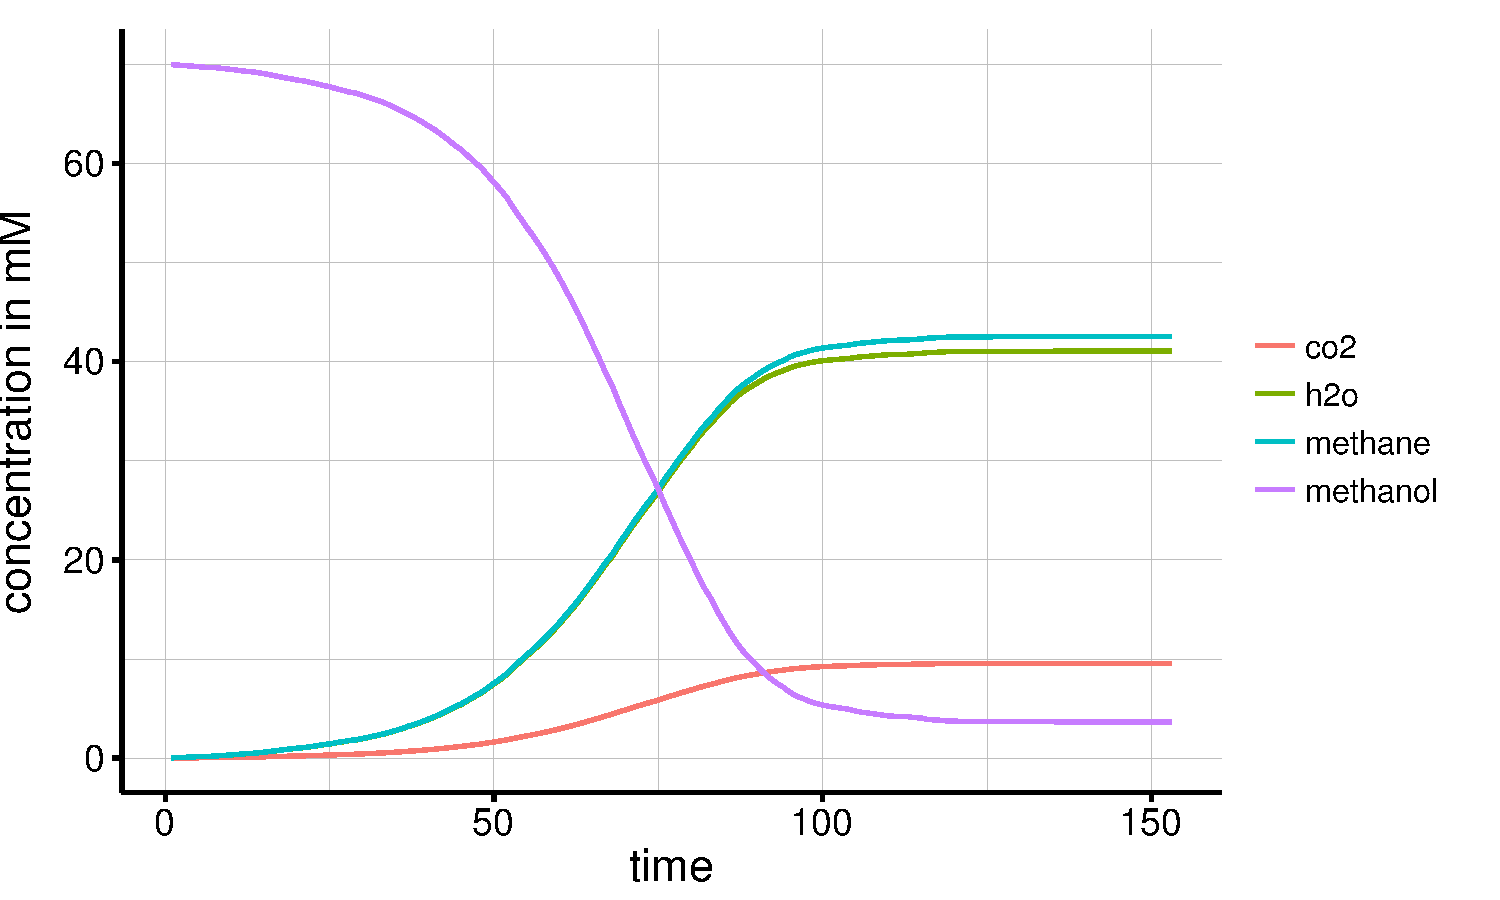
\includegraphics[scale=0.45]{../results/barkeri_20x20_seed9659_subs.pdf}
  \caption{Population dynamics of the \emph{M. barkeri} model on a $20\times20$ grid, with bacterial growth (A) and consumption/production of various metabolites (B). An initial concentration of 70\;mmol per grid cell of methanol was added to the environment. The seed of the random number generator was set to 9659.}
\end{figure}
\begin{figure}[h]
  \centering
  \subfigure[]{
    \begin{minipage}[t]{0.3\textwidth}
    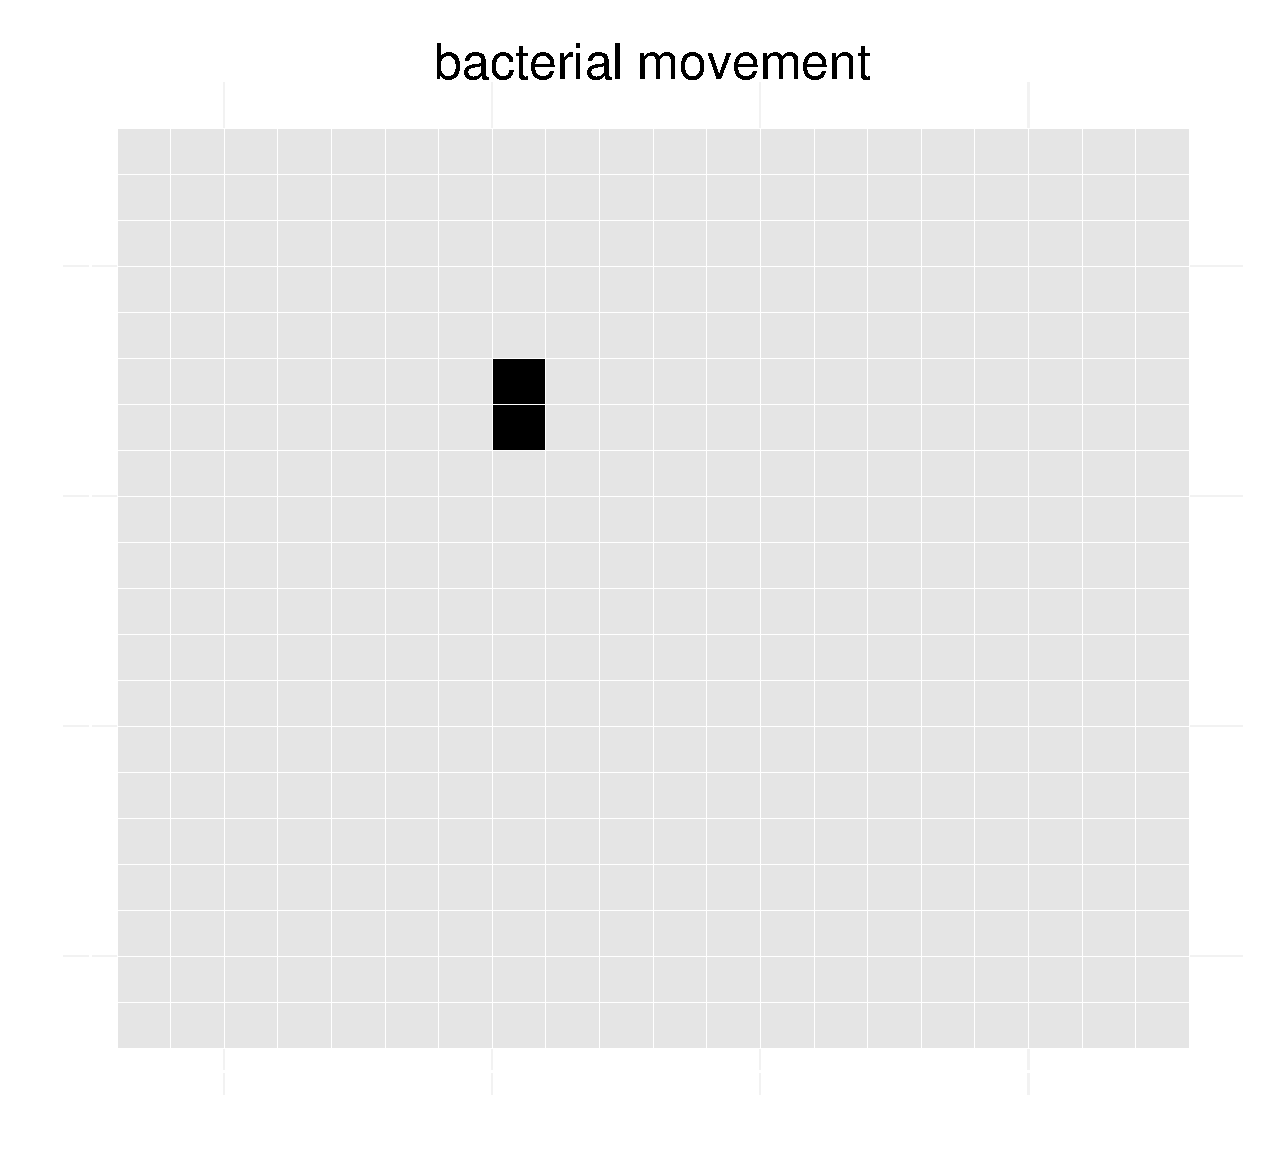
\includegraphics[width=\textwidth]{../results/barkeri_20x20_seed9659_bac10.pdf}
  \end{minipage}
  \begin{minipage}[t]{0.3\textwidth}
    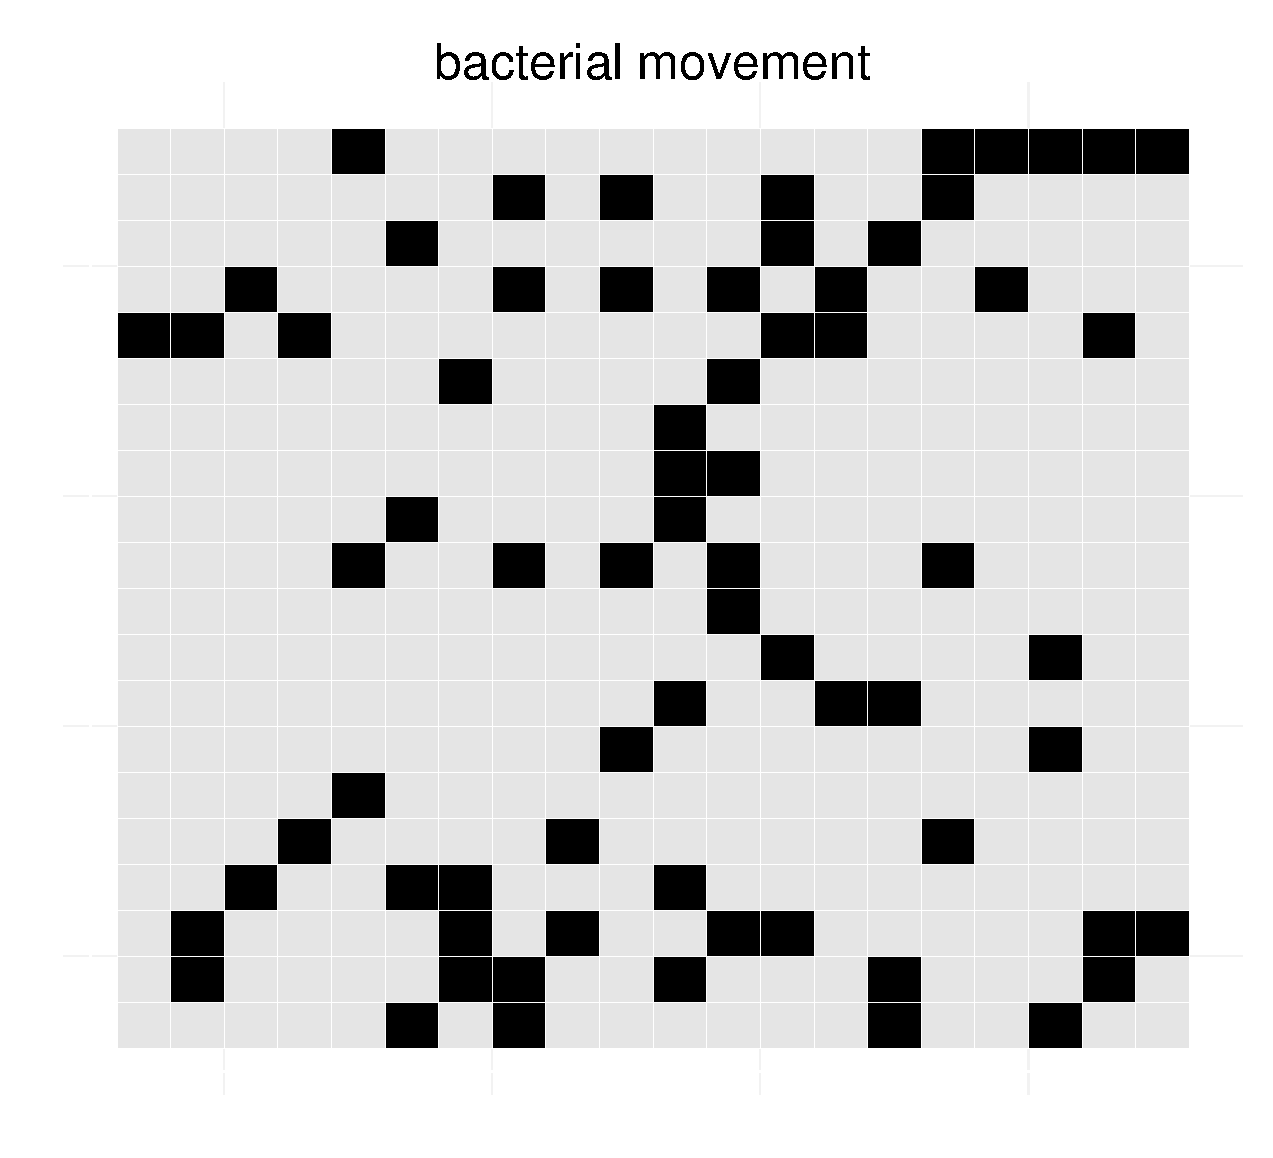
\includegraphics[width=\textwidth]{../results/barkeri_20x20_seed9659_bac100.pdf}
  \end{minipage}
  \begin{minipage}[t]{0.3\textwidth}
    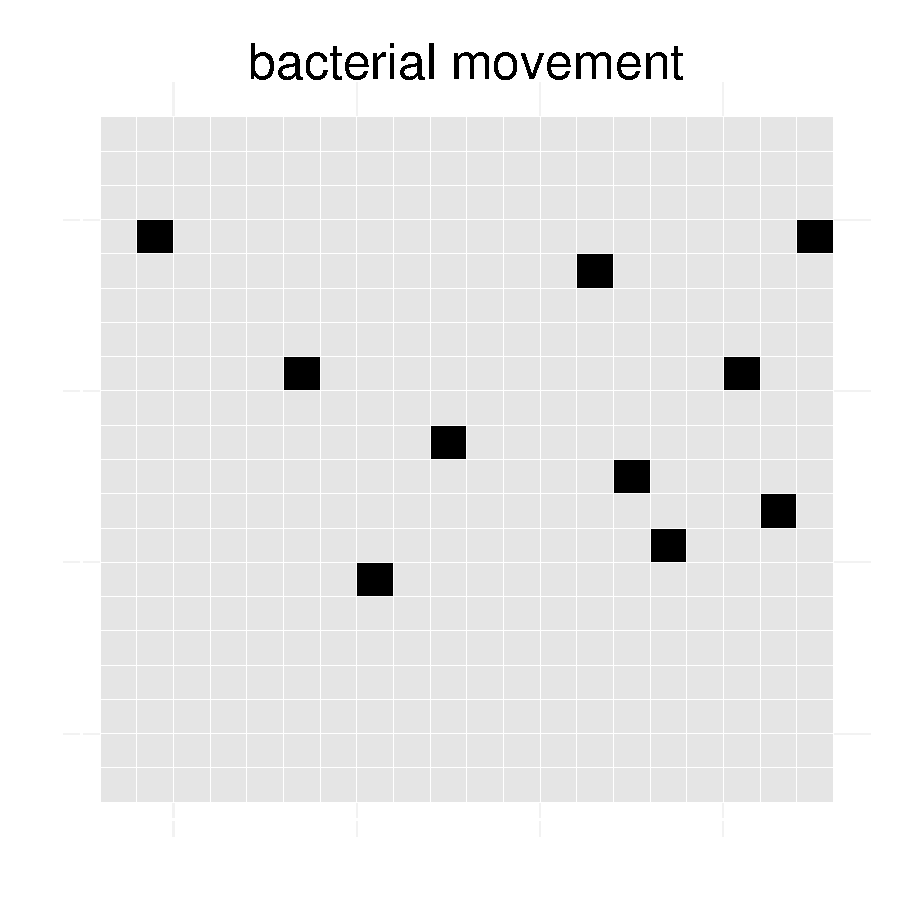
\includegraphics[width=\textwidth]{../results/barkeri_20x20_seed9659_bac130.pdf}
  \end{minipage}
  }
  \subfigure[]{
  \begin{minipage}[t]{0.3\textwidth}
    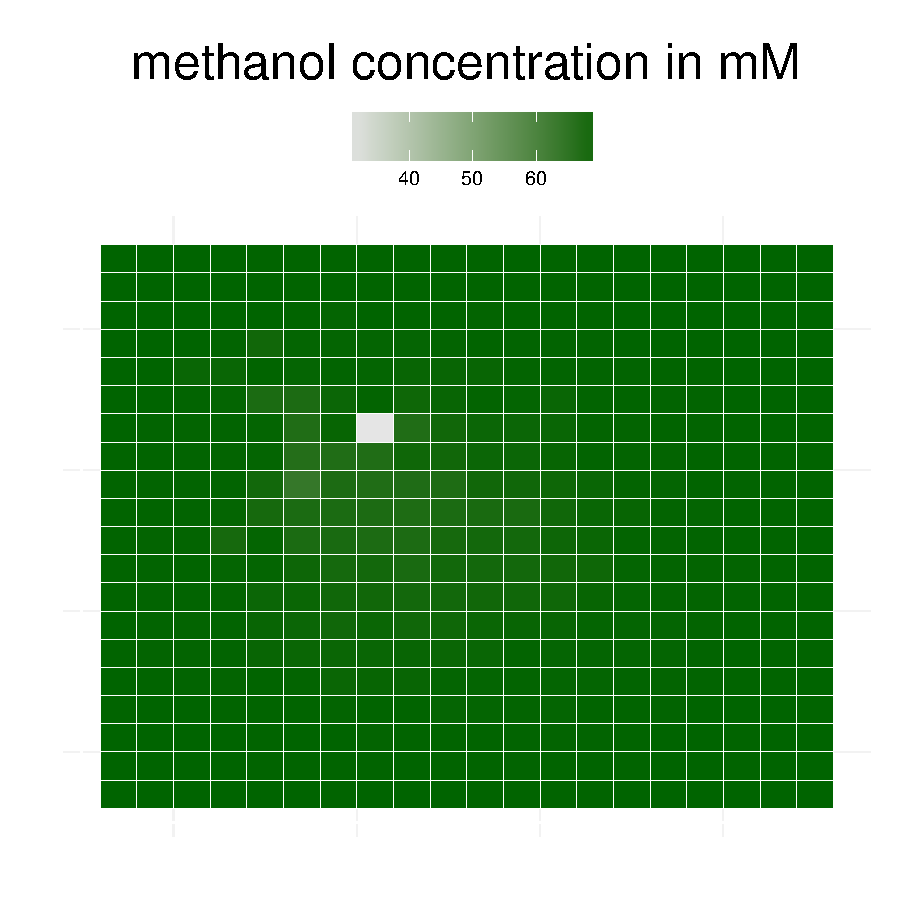
\includegraphics[width=\textwidth]{../results/barkeri_20x20_seed9659_methanol10.pdf}
  \end{minipage}
  \begin{minipage}[t]{0.3\textwidth}
    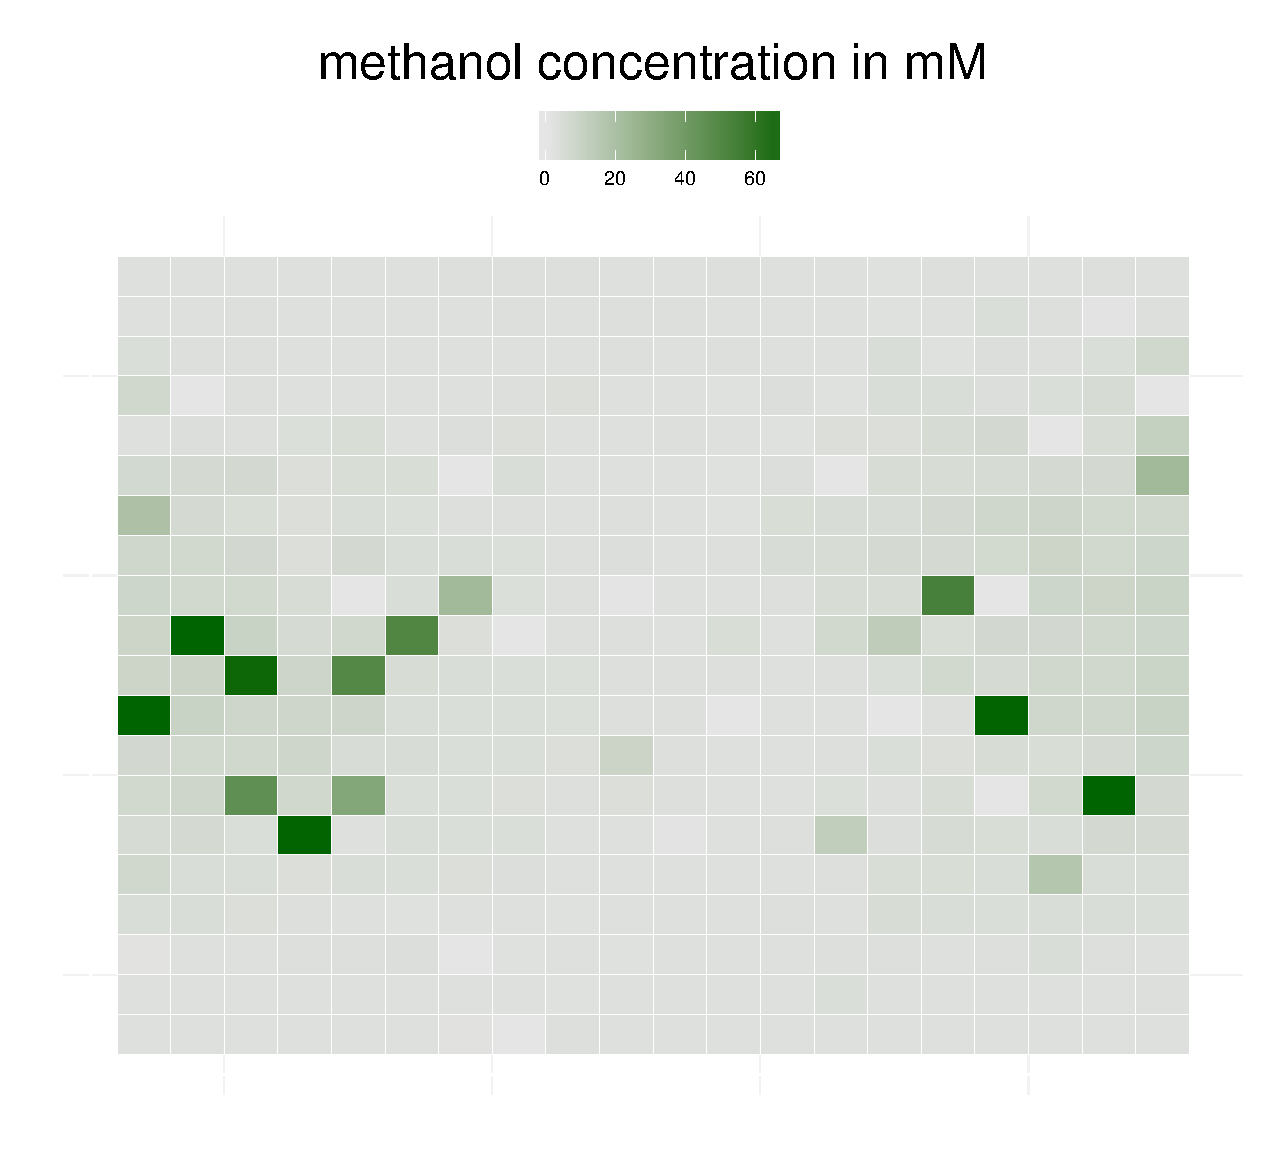
\includegraphics[width=\textwidth]{../results/barkeri_20x20_seed9659_methanol100.pdf}
  \end{minipage}
  \begin{minipage}[t]{0.3\textwidth}
    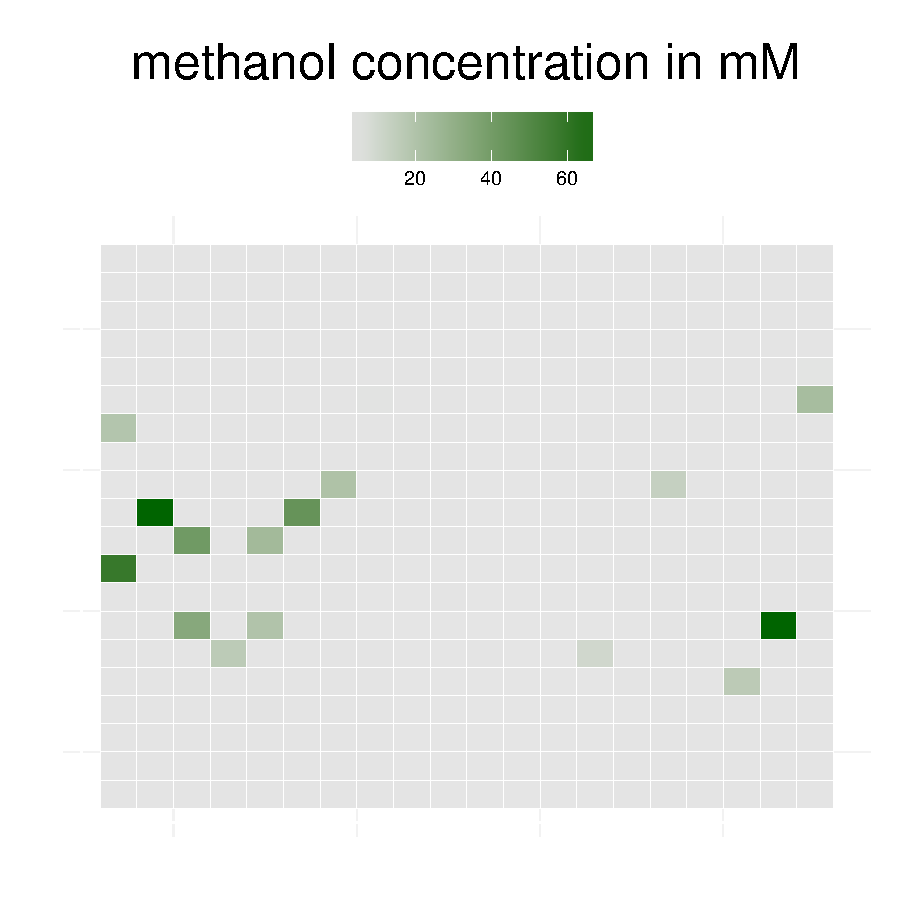
\includegraphics[width=\textwidth]{../results/barkeri_20x20_seed9659_methanol130.pdf}
  \end{minipage}
  }
  \subfigure[]{
  \begin{minipage}[t]{0.3\textwidth}
    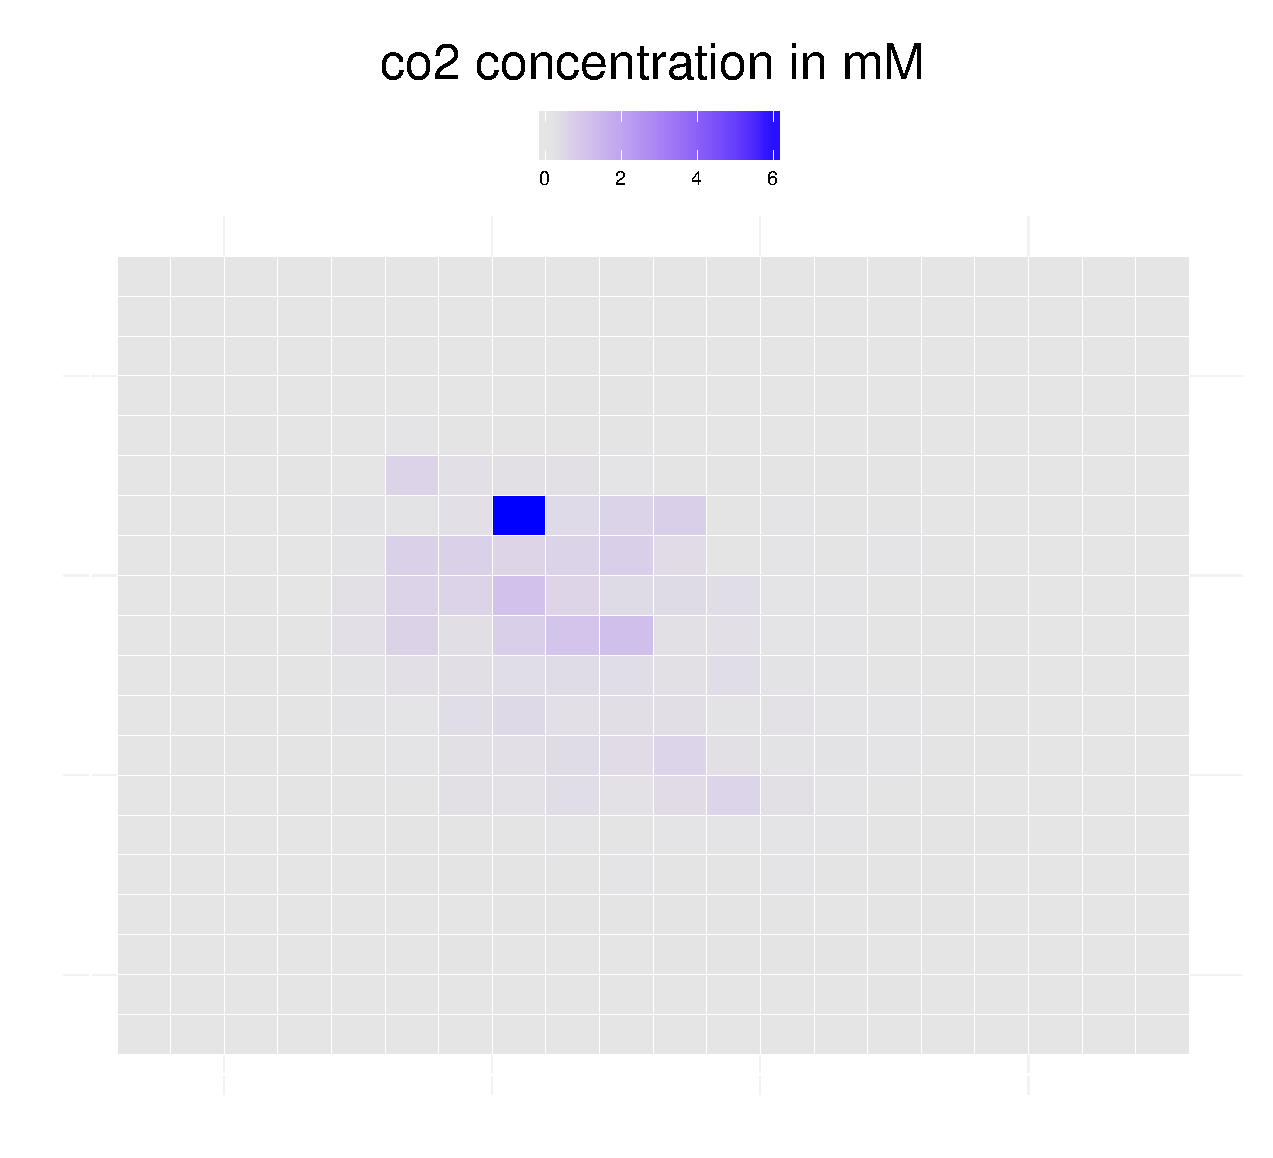
\includegraphics[width=\textwidth]{../results/barkeri_20x20_seed9659_co210.pdf}
  \end{minipage}
  \begin{minipage}[t]{0.3\textwidth}
    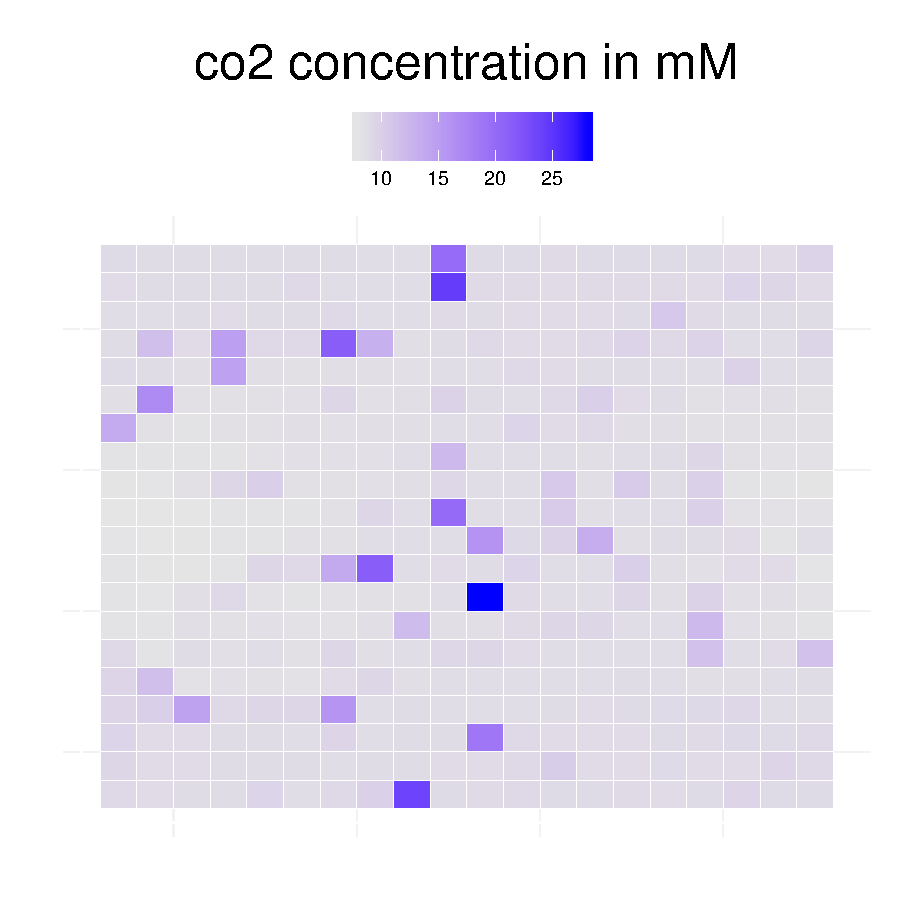
\includegraphics[width=\textwidth]{../results/barkeri_20x20_seed9659_co2100.pdf}
  \end{minipage}
  \begin{minipage}[t]{0.3\textwidth}
    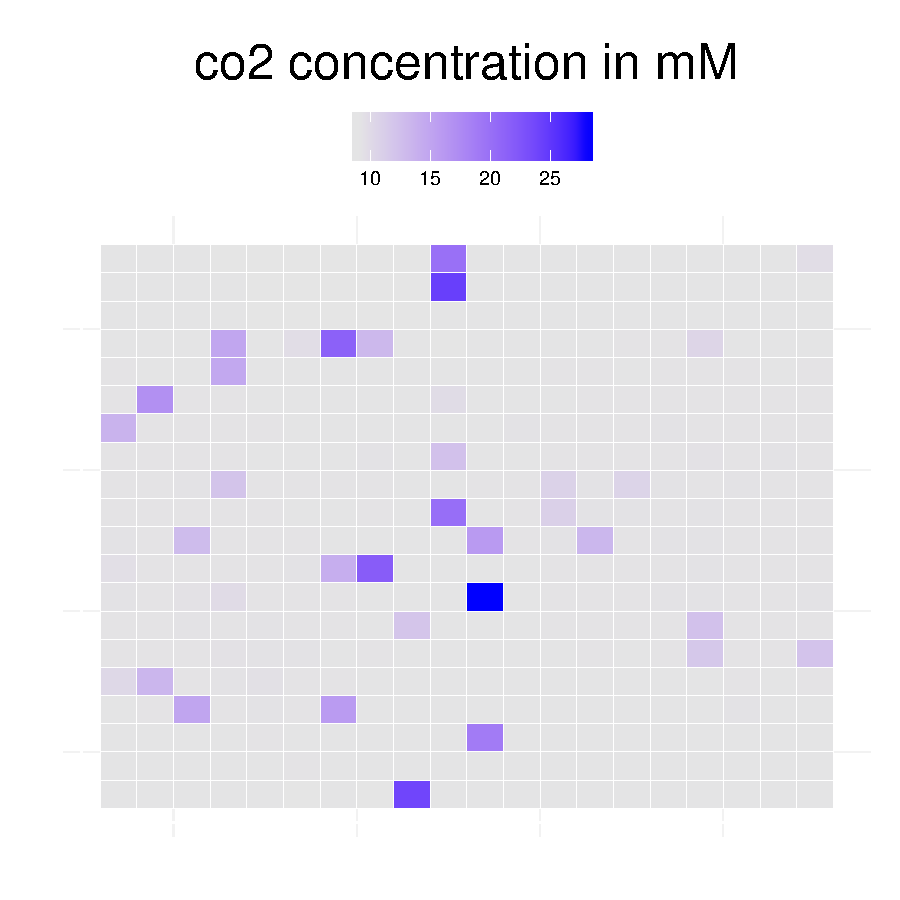
\includegraphics[width=\textwidth]{../results/barkeri_20x20_seed9659_co2130.pdf}
  \end{minipage}
  }
  \subfigure[]{
  \begin{minipage}[t]{0.3\textwidth}
    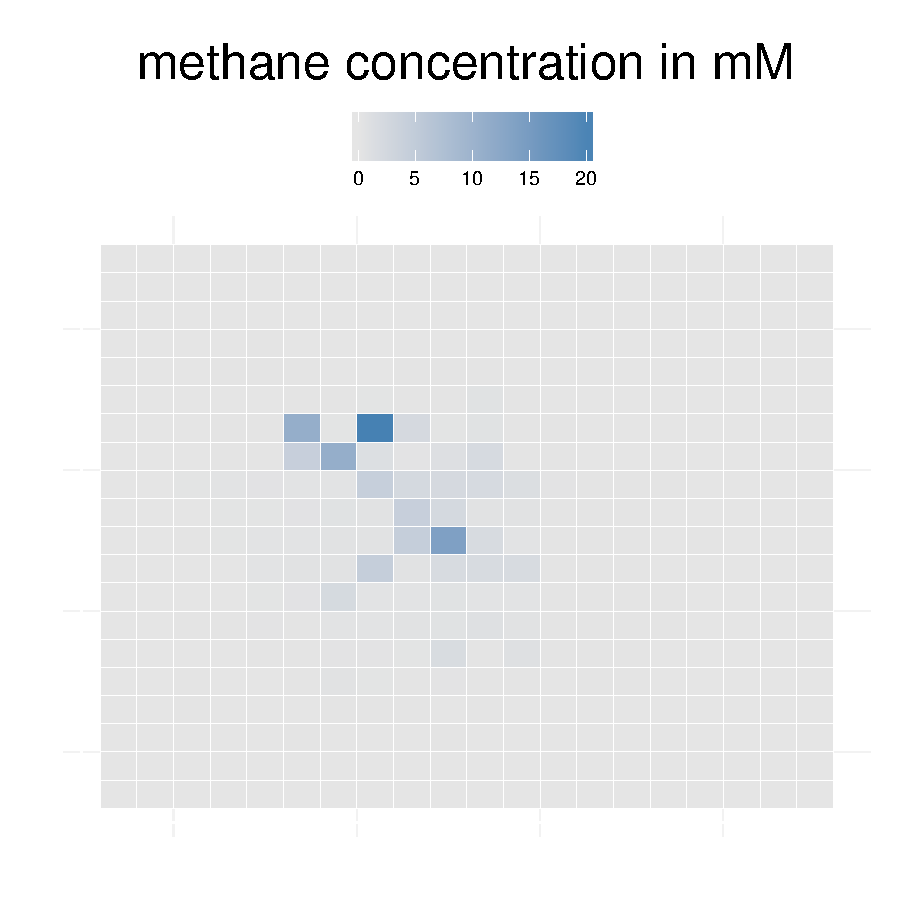
\includegraphics[width=\textwidth]{../results/barkeri_20x20_seed9659_meth10.pdf}
  \end{minipage}
  \begin{minipage}[t]{0.3\textwidth}
    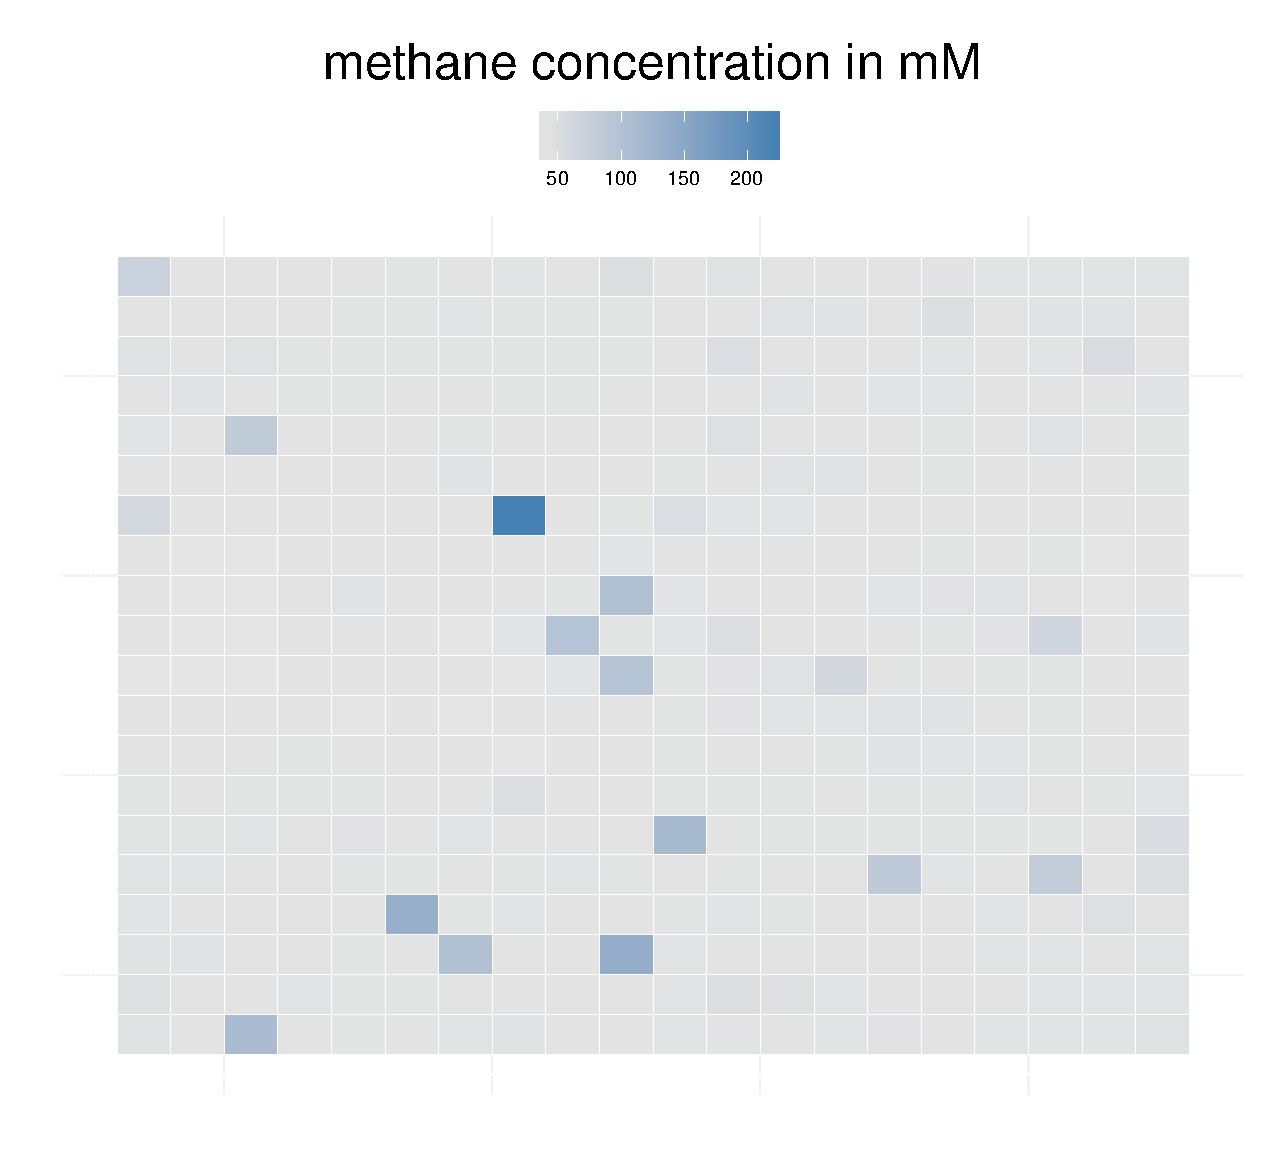
\includegraphics[width=\textwidth]{../results/barkeri_20x20_seed9659_meth100.pdf}
  \end{minipage}
  \begin{minipage}[t]{0.3\textwidth}
    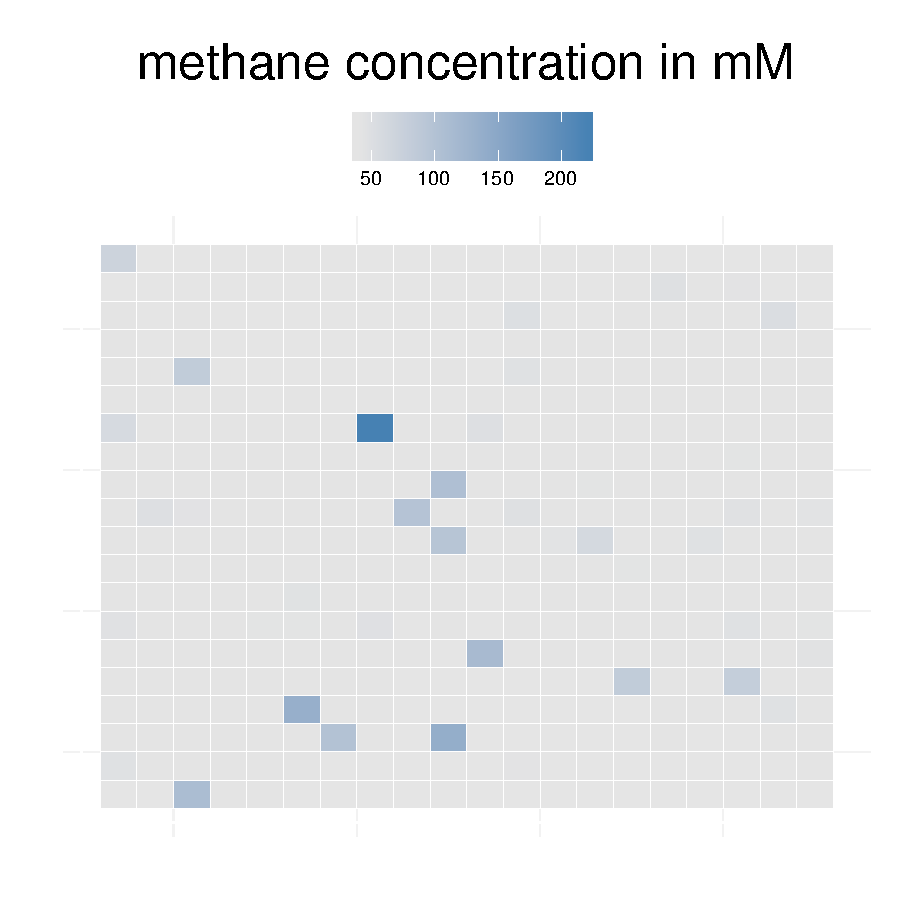
\includegraphics[width=\textwidth]{../results/barkeri_20x20_seed9659_meth130.pdf}
  \end{minipage}
  }
  \caption{Population dynamics of the \emph{M. barkeri} model on a $20\times20$ grid, with bacterial movement (A) and concentrations of methanol (B), CO$_2$ (C) and methane (D) (of time step 10, 100 and 130). The seed of the random number generator was set to 9659.}
\end{figure}

\subsubsection{\textit{Clostridium beijerinckii}}

\begin{figure}[h]
  \centering
    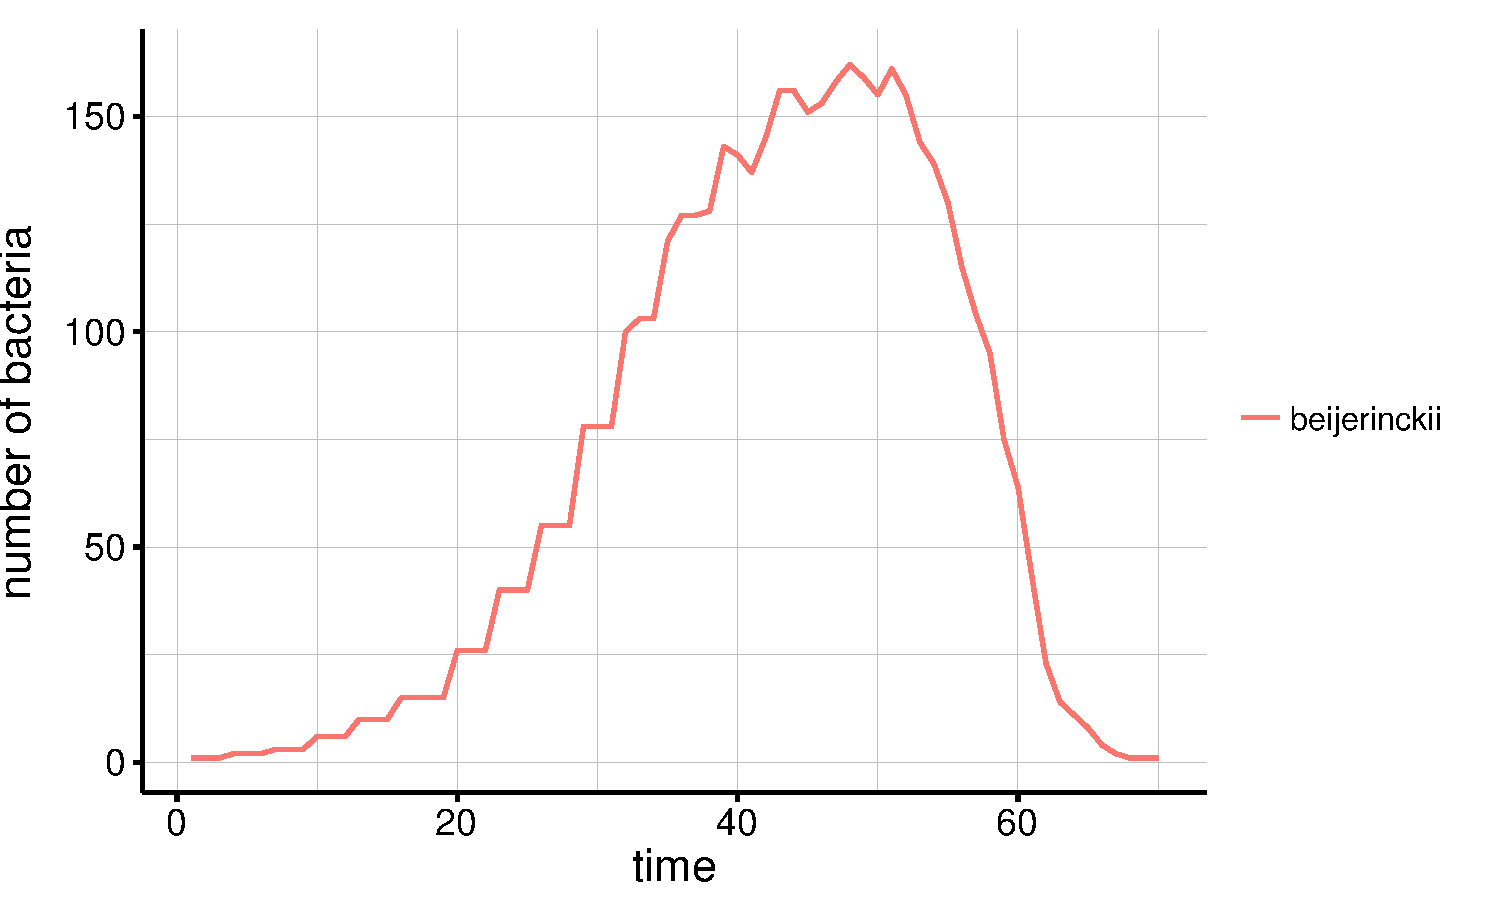
\includegraphics[scale=0.45]{../results/beijerinckii_20x20_seed943_growth.pdf}
    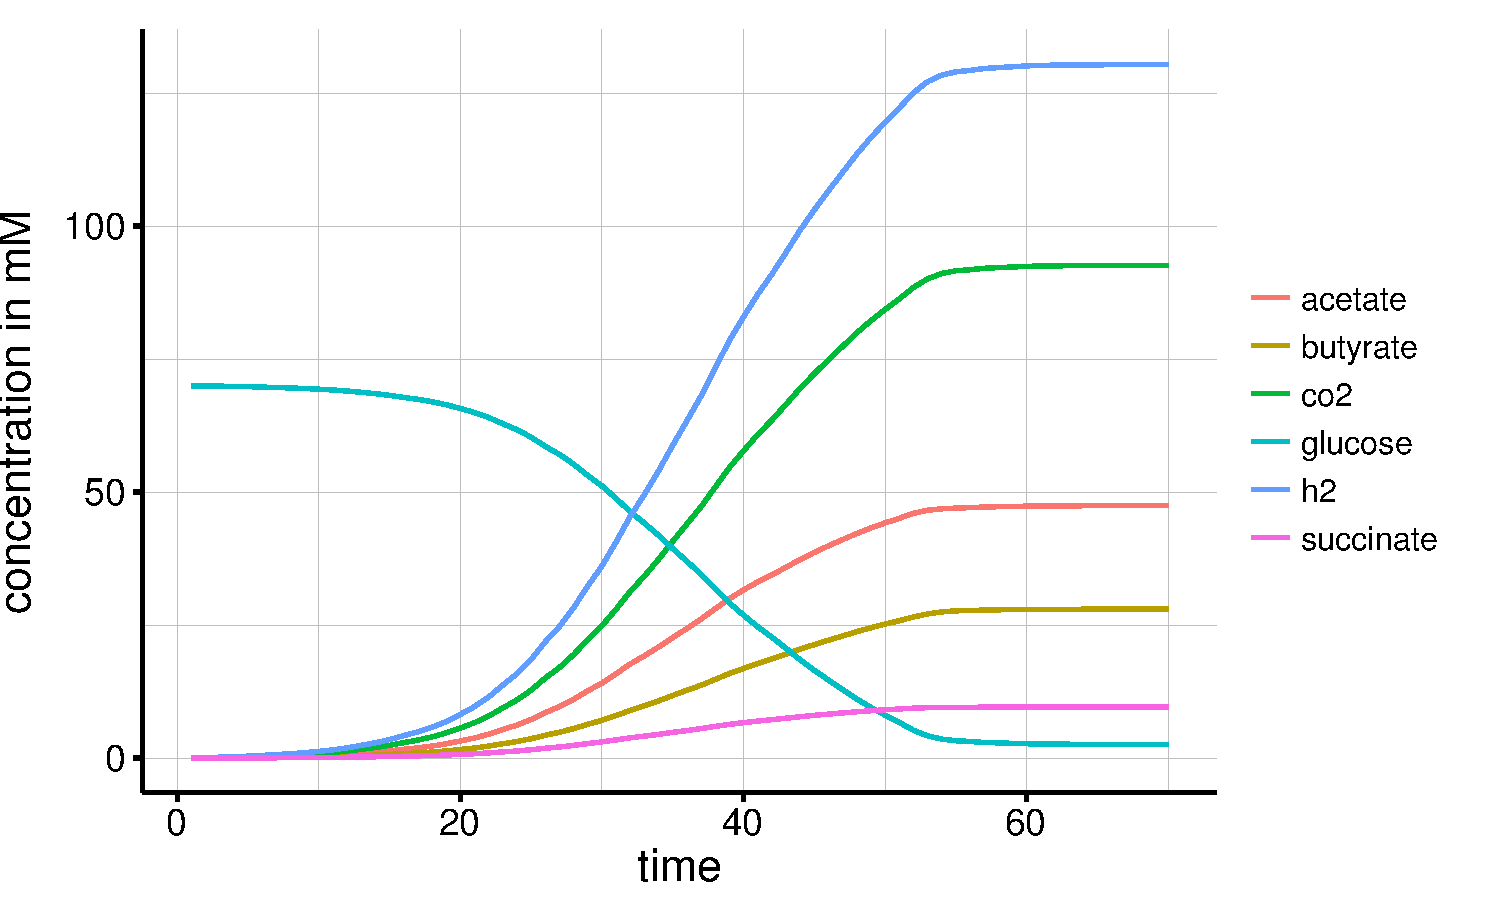
\includegraphics[scale=0.45]{../results/beijerinckii_20x20_seed943_subs.pdf}
  \caption{Population dynamics of the \emph{C. beijerinckii} model on a $20\times20$ grid, with bacterial growth (A) and consumption/production of various metabolites (B). An initial concentration of 70\;mmol per grid cell of glucose was added to the environment. The seed of the random number generator was set to 943.}
\end{figure}
\begin{figure}[h]
  \centering
  \subfigure[]{
    \begin{minipage}[t]{0.3\textwidth}
    \includegraphics[width=\textwidth]{../results/beijerinckii_20x20_seed943_bac10.pdf}
  \end{minipage}
  \begin{minipage}[t]{0.3\textwidth}
    \includegraphics[width=\textwidth]{../results/beijerinckii_20x20_seed943_bac50.pdf}
  \end{minipage}
  \begin{minipage}[t]{0.3\textwidth}
    \includegraphics[width=\textwidth]{../results/beijerinckii_20x20_seed943_bac65.pdf}
  \end{minipage}
  }
  \subfigure[]{
  \begin{minipage}[t]{0.3\textwidth}
    \includegraphics[width=\textwidth]{../results/beijerinckii_20x20_seed943_gluc10.pdf}
  \end{minipage}
  \begin{minipage}[t]{0.3\textwidth}
    \includegraphics[width=\textwidth]{../results/beijerinckii_20x20_seed943_gluc50.pdf}
  \end{minipage}
  \begin{minipage}[t]{0.3\textwidth}
    \includegraphics[width=\textwidth]{../results/beijerinckii_20x20_seed943_gluc65.pdf}
  \end{minipage}
  }
  \subfigure[]{
  \begin{minipage}[t]{0.3\textwidth}
    \includegraphics[width=\textwidth]{../results/beijerinckii_20x20_seed943_h210.pdf}
  \end{minipage}
  \begin{minipage}[t]{0.3\textwidth}
    \includegraphics[width=\textwidth]{../results/beijerinckii_20x20_seed943_h250.pdf}
  \end{minipage}
  \begin{minipage}[t]{0.3\textwidth}
    \includegraphics[width=\textwidth]{../results/beijerinckii_20x20_seed943_h265.pdf}
  \end{minipage}
  }
  \subfigure[]{
  \begin{minipage}[t]{0.3\textwidth}
    \includegraphics[width=\textwidth]{../results/beijerinckii_20x20_seed943_co210.pdf}
  \end{minipage}
  \begin{minipage}[t]{0.3\textwidth}
    \includegraphics[width=\textwidth]{../results/beijerinckii_20x20_seed943_co250.pdf}
  \end{minipage}
  \begin{minipage}[t]{0.3\textwidth}
    \includegraphics[width=\textwidth]{../results/beijerinckii_20x20_seed943_co265.pdf}
  \end{minipage}
  }
  \caption{Population dynamics of the \emph{C. beijerinckii} model on a $20\times20$ grid, with bacterial movement (A) and concentrations of glucose (B), hydrogen (C) and CO$_2$ (D) (of time step 10, 50 and 65). The seed of the random number generator was set to 943.}
\end{figure}

\subsection{Mixed communities}
\subsubsection{\textit{Escherichia coli} \& \textit{Methanosarcina barkeri}}

\begin{figure}[h]
  \centering
    \includegraphics[scale=0.45]{../results/barkeri_ecoli_20x20_seed4612_growth.pdf}
    \includegraphics[scale=0.45]{../results/barkeri_ecoli_20x20_seed4612_subs.pdf}
  \caption{Population dynamics of the joint \emph{E. coli} and \emph{M. barkeri} model on a $20\times20$ grid, with bacterial growth (A) and consumption/production of various metabolites (B). An initial concentration of 70\;mmol per grid cell of glucose and methanol was added to the environment. The seed of the random number generator was set to 4612.}
\end{figure}
\begin{figure}[h]
  \centering
  \subfigure[]{
    \begin{minipage}[t]{0.3\textwidth}
    \includegraphics[width=\textwidth]{../results/barkeri_ecoli_20x20_seed4612_bac50.pdf}
  \end{minipage}
  \begin{minipage}[t]{0.3\textwidth}
    \includegraphics[width=\textwidth]{../results/barkeri_ecoli_20x20_seed4612_bac100.pdf}
  \end{minipage}
  \begin{minipage}[t]{0.3\textwidth}
    \includegraphics[width=\textwidth]{../results/barkeri_ecoli_20x20_seed4612_bac150.pdf}
  \end{minipage}
  }
  \subfigure[]{
  \begin{minipage}[t]{0.3\textwidth}
    \includegraphics[width=\textwidth]{../results/barkeri_ecoli_20x20_seed4612_gluc50.pdf}
  \end{minipage}
  \begin{minipage}[t]{0.3\textwidth}
    \includegraphics[width=\textwidth]{../results/barkeri_ecoli_20x20_seed4612_gluc100.pdf}
  \end{minipage}
  \begin{minipage}[t]{0.3\textwidth}
    \includegraphics[width=\textwidth]{../results/barkeri_ecoli_20x20_seed4612_gluc150.pdf}
  \end{minipage}
  }
  \subfigure[]{
  \begin{minipage}[t]{0.3\textwidth}
    \includegraphics[width=\textwidth]{../results/barkeri_ecoli_20x20_seed4612_ace50.pdf}
  \end{minipage}
  \begin{minipage}[t]{0.3\textwidth}
    \includegraphics[width=\textwidth]{../results/barkeri_ecoli_20x20_seed4612_ace100.pdf}
  \end{minipage}
  \begin{minipage}[t]{0.3\textwidth}
    \includegraphics[width=\textwidth]{../results/barkeri_ecoli_20x20_seed4612_ace150.pdf}
  \end{minipage}
  }
  \subfigure[]{
  \begin{minipage}[t]{0.3\textwidth}
    \includegraphics[width=\textwidth]{../results/barkeri_ecoli_20x20_seed4612_meth50.pdf}
  \end{minipage}
  \begin{minipage}[t]{0.3\textwidth}
    \includegraphics[width=\textwidth]{../results/barkeri_ecoli_20x20_seed4612_meth100.pdf}
  \end{minipage}
  \begin{minipage}[t]{0.3\textwidth}
    \includegraphics[width=\textwidth]{../results/barkeri_ecoli_20x20_seed4612_meth150.pdf}
  \end{minipage}
  }
  \caption{Population dynamics of the joint \emph{E. coli} and \emph{M. barkeri} model on a $20\times20$ grid, with bacterial movement (A) and concentrations of glucose (B), acetate (C) and methane (D) (of time step 50, 100 and 150). The seed of the random number generator was set to 4612.}
\end{figure}

\subsubsection{\textit{Escherichia coli} \& \textit{Clostridium beijerinckii}}

\begin{figure}[h]
  \centering
    \includegraphics[scale=0.45]{../results/ecoli_beijerinckii_20x20_seed5147_growth.pdf}
    \includegraphics[scale=0.45]{../results/ecoli_beijerinckii_20x20_seed5147_subs.pdf}
  \caption{Population dynamics of the joint \emph{E. coli} and \emph{C. beijerinckii} model on a $20\times20$ grid, with bacterial growth (A) and consumption/production of various metabolites (B). An initial concentration of 70\;mmol per grid cell of glucose was added to the environment. The seed of the random number generator was set to 5147.}
\end{figure}
\begin{figure}[h]
  \centering
  \subfigure[]{
    \begin{minipage}[t]{0.3\textwidth}
    \includegraphics[width=\textwidth]{../results/ecoli_beijerinckii_20x20_seed5147_bac10.pdf}
  \end{minipage}
  \begin{minipage}[t]{0.3\textwidth}
    \includegraphics[width=\textwidth]{../results/ecoli_beijerinckii_20x20_seed5147_bac55.pdf}
  \end{minipage}
  \begin{minipage}[t]{0.3\textwidth}
    \includegraphics[width=\textwidth]{../results/ecoli_beijerinckii_20x20_seed5147_bac75.pdf}
  \end{minipage}
  }
  \subfigure[]{
  \begin{minipage}[t]{0.3\textwidth}
    \includegraphics[width=\textwidth]{../results/ecoli_beijerinckii_20x20_seed5147_gluc10.pdf}
  \end{minipage}
  \begin{minipage}[t]{0.3\textwidth}
    \includegraphics[width=\textwidth]{../results/ecoli_beijerinckii_20x20_seed5147_gluc55.pdf}
  \end{minipage}
  \begin{minipage}[t]{0.3\textwidth}
    \includegraphics[width=\textwidth]{../results/ecoli_beijerinckii_20x20_seed5147_gluc75.pdf}
  \end{minipage}
  }
  \subfigure[]{
  \begin{minipage}[t]{0.3\textwidth}
    \includegraphics[width=\textwidth]{../results/ecoli_beijerinckii_20x20_seed5147_h210.pdf}
  \end{minipage}
  \begin{minipage}[t]{0.3\textwidth}
    \includegraphics[width=\textwidth]{../results/ecoli_beijerinckii_20x20_seed5147_h255.pdf}
  \end{minipage}
  \begin{minipage}[t]{0.3\textwidth}
    \includegraphics[width=\textwidth]{../results/ecoli_beijerinckii_20x20_seed5147_h275.pdf}
  \end{minipage}
  }
  \subfigure[]{
  \begin{minipage}[t]{0.3\textwidth}
    \includegraphics[width=\textwidth]{../results/ecoli_beijerinckii_20x20_seed5147_etoh10.pdf}
  \end{minipage}
  \begin{minipage}[t]{0.3\textwidth}
    \includegraphics[width=\textwidth]{../results/ecoli_beijerinckii_20x20_seed5147_etoh55.pdf}
  \end{minipage}
  \begin{minipage}[t]{0.3\textwidth}
    \includegraphics[width=\textwidth]{../results/ecoli_beijerinckii_20x20_seed5147_etoh75.pdf}
  \end{minipage}
  }
  \caption{Population dynamics of the joint \emph{E. coli} and \emph{C. beijerinckii} model on a $20\times20$ grid, with bacterial movement (A) and concentrations of glucose (B), hydrogen (C) and ethanol (D) (of time step 10, 55 and 75). The seed of the random number generator was set to 5147.}
\end{figure}

\subsubsection{\textit{Clostridium beijerinckii} \& \textit{Methanosarcina barkeri}}

\begin{figure}[h]
  \centering
    \includegraphics[scale=0.45]{../results/barkeri_beijerinckii_20x20_seed6764_growth.pdf}
    \includegraphics[scale=0.45]{../results/barkeri_beijerinckii_20x20_seed6764_subs.pdf}
  \caption{Population dynamics of the joint \emph{M. barkeri} and \emph{C. beijerinckii} model on a $20\times20$ grid, with bacterial growth (A) and consumption/production of various metabolites (B). An initial concentration of 70\;mmol per grid cell of glucose was added to the environment. The seed of the random number generator was set to 6764.}
\end{figure}
\begin{figure}[h]
  \centering
  \subfigure[]{
    \begin{minipage}[t]{0.3\textwidth}
    \includegraphics[width=\textwidth]{../results/barkeri_beijerinckii_20x20_seed6764_bac50.pdf}
  \end{minipage}
  \begin{minipage}[t]{0.3\textwidth}
    \includegraphics[width=\textwidth]{../results/barkeri_beijerinckii_20x20_seed6764_bac100.pdf}
  \end{minipage}
  \begin{minipage}[t]{0.3\textwidth}
    \includegraphics[width=\textwidth]{../results/barkeri_beijerinckii_20x20_seed6764_bac150.pdf}
  \end{minipage}
  }
  \subfigure[]{
  \begin{minipage}[t]{0.3\textwidth}
    \includegraphics[width=\textwidth]{../results/barkeri_beijerinckii_20x20_seed6764_gluc50.pdf}
  \end{minipage}
  \begin{minipage}[t]{0.3\textwidth}
    \includegraphics[width=\textwidth]{../results/barkeri_beijerinckii_20x20_seed6764_gluc100.pdf}
  \end{minipage}
  \begin{minipage}[t]{0.3\textwidth}
    \includegraphics[width=\textwidth]{../results/barkeri_beijerinckii_20x20_seed6764_gluc150.pdf}
  \end{minipage}
  }
  \subfigure[]{
  \begin{minipage}[t]{0.3\textwidth}
    \includegraphics[width=\textwidth]{../results/barkeri_beijerinckii_20x20_seed6764_h250.pdf}
  \end{minipage}
  \begin{minipage}[t]{0.3\textwidth}
    \includegraphics[width=\textwidth]{../results/barkeri_beijerinckii_20x20_seed6764_h2100.pdf}
  \end{minipage}
  \begin{minipage}[t]{0.3\textwidth}
    \includegraphics[width=\textwidth]{../results/barkeri_beijerinckii_20x20_seed6764_h2150.pdf}
  \end{minipage}
  }
  \subfigure[]{
  \begin{minipage}[t]{0.3\textwidth}
    \includegraphics[width=\textwidth]{../results/barkeri_beijerinckii_20x20_seed6764_meth50.pdf}
  \end{minipage}
  \begin{minipage}[t]{0.3\textwidth}
    \includegraphics[width=\textwidth]{../results/barkeri_beijerinckii_20x20_seed6764_meth100.pdf}
  \end{minipage}
  \begin{minipage}[t]{0.3\textwidth}
    \includegraphics[width=\textwidth]{../results/barkeri_beijerinckii_20x20_seed6764_meth150.pdf}
  \end{minipage}
  }
  \caption{Dynamics of the joint \emph{M. barkeri} and \emph{C. beijerinckii} model on a $20\times20$ grid, with bacterial movement (A) and concentrations of glucose (B), hydrogen (C) and methanol (D) (time step 50, 100 and 150). The seed of the random number generator was set to 6764.}
\end{figure}

%\subsection{Spatial and time-wise heterogeneity}
%\subsubsection{Substrate gradients}
%\subsubsection{Delayed bacterial input}
